%%%%%%%%%%%%%%%%%%%%%%%%%%%%%%%%%%%%%%%%%
% Beamer Presentation
% LaTeX Template
% Version 2.0 (March 8, 2022)
%
% This template originates from:
% https://www.LaTeXTemplates.com
%
% Author:
% Vel (vel@latextemplates.com)
%
% License:
% CC BY-NC-SA 4.0 (https://creativecommons.org/licenses/by-nc-sa/4.0/)
%
%%%%%%%%%%%%%%%%%%%%%%%%%%%%%%%%%%%%%%%%%

%----------------------------------------------------------------------------------------
%	PACKAGES AND OTHER DOCUMENT CONFIGURATIONS
%----------------------------------------------------------------------------------------

\documentclass[
	11pt, % Set the default font size, options include: 8pt, 9pt, 10pt, 11pt, 12pt, 14pt, 17pt, 20pt
	%t, % Uncomment to vertically align all slide content to the top of the slide, rather than the default centered
	%aspectratio=169, % Uncomment to set the aspect ratio to a 16:9 ratio which matches the aspect ratio of 1080p and 4K screens and projectors
]{beamer}

%\graphicspath{{Images/}{./}} % Specifies where to look for included images (trailing slash required)

\usepackage{booktabs} % Allows the use of \toprule, \midrule and \bottomrule for better rules in tables
\usepackage{amsmath}
\usepackage{subfig}
\usepackage{graphicx}
\usepackage{lipsum}
\usepackage{caption}
\captionsetup[subfloat]{captionskip=1pt}

%----------------------------------------------------------------------------------------
%	SELECT LAYOUT THEME
%----------------------------------------------------------------------------------------

% Beamer comes with a number of default layout themes which change the colors and layouts of slides. Below is a list of all themes available, uncomment each in turn to see what they look like.

%\usetheme{default}
%\usetheme{AnnArbor}
%\usetheme{Antibes}
%\usetheme{Bergen}
%\usetheme{Berkeley}
%\usetheme{Berlin}
%\usetheme{Boadilla}
%\usetheme{CambridgeUS}
%\usetheme{Copenhagen}
%\usetheme{Darmstadt}
%\usetheme{Dresden}
%\usetheme{Frankfurt}
%\usetheme{Goettingen}
%\usetheme{Hannover}
%\usetheme{Ilmenau}
%\usetheme{JuanLesPins}
%\usetheme{Luebeck}
\usetheme{Madrid}
%\usetheme{Malmoe}
%\usetheme{Marburg}
%\usetheme{Montpellier}
%\usetheme{PaloAlto}
%\usetheme{Pittsburgh}
%\usetheme{Rochester}
%\usetheme{Singapore}
%\usetheme{Szeged}
%\usetheme{Warsaw}

%----------------------------------------------------------------------------------------
%	SELECT COLOR THEME
%----------------------------------------------------------------------------------------

% Beamer comes with a number of color themes that can be applied to any layout theme to change its colors. Uncomment each of these in turn to see how they change the colors of your selected layout theme.

%\usecolortheme{albatross}
%\usecolortheme{beaver}
%\usecolortheme{beetle}
%\usecolortheme{crane}
%\usecolortheme{dolphin}
%\usecolortheme{dove}
%\usecolortheme{fly}
%\usecolortheme{lily}
%\usecolortheme{monarca}
%\usecolortheme{seagull}
%\usecolortheme{seahorse}
%\usecolortheme{spruce}
%\usecolortheme{whale}
%\usecolortheme{wolverine}

%----------------------------------------------------------------------------------------
%	SELECT FONT THEME & FONTS
%----------------------------------------------------------------------------------------

% Beamer comes with several font themes to easily change the fonts used in various parts of the presentation. Review the comments beside each one to decide if you would like to use it. Note that additional options can be specified for several of these font themes, consult the beamer documentation for more information.

\usefonttheme{default} % Typeset using the default sans serif font
%\usefonttheme{serif} % Typeset using the default serif font (make sure a sans font isn't being set as the default font if you use this option!)
%\usefonttheme{structurebold} % Typeset important structure text (titles, headlines, footlines, sidebar, etc) in bold
%\usefonttheme{structureitalicserif} % Typeset important structure text (titles, headlines, footlines, sidebar, etc) in italic serif
%\usefonttheme{structuresmallcapsserif} % Typeset important structure text (titles, headlines, footlines, sidebar, etc) in small caps serif
%------------------------------------------------

\usepackage{mathptmx} % Use the Times font for serif text
%\usepackage{palatino} % Use the Palatino font for serif text

%\usepackage{helvet} % Use the Helvetica font for sans serif text
\usepackage[default]{opensans} % Use the Open Sans font for sans serif text
%\usepackage[default]{FiraSans} % Use the Fira Sans font for sans serif text
%\usepackage[default]{lato} % Use the Lato font for sans serif text

%----------------------------------------------------------------------------------------
%	SELECT INNER THEME
%----------------------------------------------------------------------------------------

% Inner themes change the styling of internal slide elements, for example: bullet points, blocks, bibliography entries, title pages, theorems, etc. Uncomment each theme in turn to see what changes it makes to your presentation.

%\useinnertheme{default}
\useinnertheme{circles}
%\useinnertheme{rectangles}
%\useinnertheme{rounded}
%\useinnertheme{inmargin}

%----------------------------------------------------------------------------------------
%	SELECT OUTER THEME
%----------------------------------------------------------------------------------------

% Outer themes change the overall layout of slides, such as: header and footer lines, sidebars and slide titles. Uncomment each theme in turn to see what changes it makes to your presentation.

%\useoutertheme{default}
%\useoutertheme{infolines}
%\useoutertheme{miniframes}
%\useoutertheme{smoothbars}
%\useoutertheme{sidebar}
%\useoutertheme{split}
%\useoutertheme{shadow}
%\useoutertheme{tree}
%\useoutertheme{smoothtree}

%\setbeamertemplate{footline} % Uncomment this line to remove the footer line in all slides
%\setbeamertemplate{footline}[page number] % Uncomment this line to replace the footer line in all slides with a simple slide count

%\setbeamertemplate{navigation symbols}{} % Uncomment this line to remove the navigation symbols from the bottom of all slides

%----------------------------------------------------------------------------------------
%	PRESENTATION INFORMATION
%----------------------------------------------------------------------------------------
\beamertemplatenavigationsymbolsempty
%\setbeameroption{show notes on second screen=right}
%\setbeameroption{show only notes}
\setbeamercolor{note page}{bg=white}
\setbeamercolor{note title}{bg=white}
\setbeamercolor{note date}{fg=white}
\newcommand{\bra}[1]{<#1|}
\newcommand{\ket}[1]{|#1>}
\newcommand{\expval}[2]{<#2|#1|#2>}
\newcommand{\laplace}{\Delta}
\newcommand{\diag}{\text{diag}}
\newcommand{\ftk}[3]{\frac{1}{(2\pi)^3}\int d#2\ #3 e^{i(#1#2)}}
\newcommand{\ftkvec}[3]{\frac{1}{(2\pi)^3}\int d#2\ #3 e^{i#1\cdot#2}}
\newcommand{\ftr}[3]{\int d#2\ #3 e^{-i(#1\cdot#2)}}
\newcommand{\vr}{\vec{r}}
\newcommand{\vR}{\vec{R}}
\newcommand{\vq}{\vec{q}}
\newcommand{\vk}{\vec{k}}
\newcommand{\vrp}{\vec{r'}}
\newcommand{\vkp}{\vec{k'}}
\newcommand{\E}{\mathcal{E}}
\newcommand{\dos}{N}
\newcommand{\schr}{Schr\"odingerova Rovnica}
\newcommand{\insertgraph}[2]{
    \begin{figure}[H]
        \centering
        \includegraphics[angle=-90,origin=c,scale=0.5,trim={1cm 0 1cm 0},clip]{grafy/#1}
        \vspace{-22mm}
        \caption{#2}
        \label{fig:#1}
    \end{figure}
}


\title[Diplomová práca]{ Hustota elektrónových stavov v kove so slabým disorderom a slabou elektrón-elektrónovou interakciou: Jav Altshulera-Aronova} % The short title in the optional parameter appears at the bottom of every slide, the full title in the main parameter is only on the title page

\subtitle{Diplomová Práca} % Presentation subtitle, remove this command if a subtitle isn't required

\author[Matúš Jenča]{Matúš Jenča} % Presenter name(s), the optional parameter can contain a shortened version to appear on the bottom of every slide, while the main parameter will appear on the title slide

\institute[FMFI UK]{Fakulta matematiky, Fyziky a Informatiky } % Your institution, the optional parameter can be used for the institution shorthand and will appear on the bottom of every slide after author names, while the required parameter is used on the title slide and can include your email address or additional information on separate lines

\date[\today]{\today  \\
\tiny
\vspace{10mm}
Vedúci práce:  Doc. RNDr. Martin Moško, DrSc. \\
Konzultant: RNDr. Antónia Mošková, CSc. \\
\normalsize} % Presentation date or conference/meeting name, the optional parameter can contain a shortened version to appear on the bottom of every slide, while the required parameter value is output to the title slide

%----------------------------------------------------------------------------------------

\begin{document}

%----------------------------------------------------------------------------------------
%	TITLE SLIDE
%----------------------------------------------------------------------------------------

\begin{frame}
	\titlepage % Output the title slide, automatically created using the text entered in the PRESENTATION INFORMATION block above
\end{frame}

%----------------------------------------------------------------------------------------
%	TABLE OF CONTENTS SLIDE
%----------------------------------------------------------------------------------------

% The table of contents outputs the sections and subsections that appear in your presentation, specified with the standard \section and \subsection commands. You may either display all sections and subsections on one slide with \tableofcontents, or display each section at a time on subsequent slides with \tableofcontents[pausesections]. The latter is useful if you want to step through each section and mention what you will discuss.

\begin{frame}
	\frametitle{Obsah} % Slide title, remove this command for no title
	\begin{itemize}
	\item Interagujúce elektróny v čistom kove: Hartreeho - Fockova aproximácia pre model želé
	\item Elektrón-elektrónová interakcia v kove s disorderom : Jav Altshulera - Aronovova
	\item Meranie hustoty stavov v kove s disorderom metódou tunelovej spektroskopie
	\item Altshuler - Aronovov jav, rozšírenie teórie na energie $|\E - \E_F| \gtrsim \hbar/\tau$
	\item Výsledky a ich diskusia
	\end{itemize}
\end{frame}
\begin{frame}

\note{Najprv definujeme základné pojmy na probléme neinteragujúcich elektrónov.
 Pre neinteragujúci elektrón máme Schr\"odingerovu rovnicu voľnej častice,
ktorej riešením je DeBroglieho rovinná vlna \eqref{eq:fp}.
Energia neinteragujúceho elektrónu je daná parabolickým disperzným zákonom.
Pre koncentráciu  elektrónov platí vzťah \eqref{eq:N integral sfercky}
}

\frametitle{Interagujúce elektróny v čistom kove: Hartreeho - Fockova aproximácia pre model želé}
\begin{itemize}
\item Pre neinteragujúci elektrón máme Schr\"odingerovu rovnicu voľnej častice,
ktorej riešením je DeBroglieho rovinná vlna
\begin{equation}
\label{eq:fp}
 \Psi(\vec r,t)=\sqrt{\frac{1}{V}}e^{i(\vec k\cdot\vec r-\frac{E(k)t}{\hbar})} \text{,}
\end{equation}
\item Energia voľnej častice je $E=\frac{\hbar^2k^2}{2m}$
\item Pre koncentráciu  elektrónov platí

\begin{equation}
 \label{eq:N integral sfercky}
 n_e \equiv \frac{N}{L_xL_yL_z} = 2 \frac{1}{8\pi^3} \int_0^{2\pi} d\phi \int_0^{\pi}  d\theta \sin{\theta} \int_0^{\infty} dk\ k^2 f(k)  \text{,}
\end{equation}
kde $f(k)$ je Fermiho distribúcia.
\end{itemize}
\end{frame}
\begin{frame}

\note{ Po integrovaní cez $\phi$ a $\theta$ a zámene premenných za energiu definujeme hustotu stavov $\rho(E)$.
Pre konkrétny prípad voľnej častice je hustota stavov úmerná odmocnine z energie.  Maximálne obsadené stavy  neinteragujúcich elektrónov pri $T=0$ budú na Fermiho Sfére s polomerom $k_f$ a Fermiho energiou $E_f$}

\begin{itemize}
\item Po úpravách \eqref{eq:N integral sfercky} definujeme hustotu stavov $\rho(E)$
\begin{equation}
 \label{eq:N integral sfer energ}
 n_e =   \int_0^{\infty}dE\rho(E)\ f(E) \ \ \text{kde}\ \ \rho(E)=\frac{1}{\pi^2} \frac{dk}{dE} k^2  \ \text{,}
\end{equation}
\item pre voľné častice 
\begin{equation}
 \label{eq:rho_par}
 \rho(E)=\frac{1}{2\pi^2}{(2 m_e/\hbar^2)}^{3/2} \sqrt{E} \text{.}
\end{equation}
\item pri $T=0$ elektróny obsadzujú stavy vo vnútri Fermiho sféry. Polomer Fermiho sféry je Fermiho vlnový vektor
\begin{equation}
 \label{eq:kf}
 k_F=(3\pi^2 n_e)^{\frac{1}{3}}\text{,}
\end{equation}
\item energia na Fermiho sfére (Fermiho Energia) je
\begin{equation}
 \label{eq:ef}
 E_f=\frac{\hbar^2 k_f^2}{2m_e}=\frac{\hbar^2(3\pi^2 n_e)^{\frac{2}{3}}  }{2m_e} \text{.}
\end{equation}
\end{itemize}
\end{frame}
\begin{frame}
\note{Po započítaní vzájomnej interakcie elektrónov (e-e interakciu) a interakciu s iónmi dostaneme mnohočasticový Hamiltonián. Sch. R. s hamiltoniánom \eqref{eq:hrtf_ham} sa nedá exaktne riešiť ani anlyticky, ani numericky, riešime ju teda v Hartree-Fockovom priblížení variačnou metódou, kde vlnové funkcie $\Psi$ hľadáme v tvare Slatterovho determinantu \eqref{eq:slatter}. Slatterov determinant zahŕňa výmenný efekt.}

\begin{itemize}
\item Mnohočasticový Hamiltonián elektrónov ktoré interagujú s mriežkou jednonásobne ionizovaných iónov a vzájomne cez Coulombovskú interakciu 
\begin{equation}
\label{eq:hrtf_ham}
\hat{H}=\sum_i [ \frac{-\hbar^2}{2m}\laplace_i  -\sum_j\frac{e^2}{4\pi \epsilon_0}{\frac{1}{|\vr_i-\vR_j|}} +\frac{1}{2}\sum_{j\neq i}\frac{e^2}{4\pi\epsilon_0}\frac{1}{|\vr_i-\vr_j|} ]
\end{equation}
\item Riešenie Sch. R. s hamiltoniánom \eqref{eq:hrtf_ham} v Hartree-Fockovom priblížení variačnou metódou
\begin{equation}
\label{eq:erg_func}
E[\Psi^*]=\expval{H}{\Psi}
\end{equation}
\item vlnové funkcie $\Psi$  v tvare Slaterovho determinantu 
\begin{equation}
\label{eq:slatter}
\Psi(\vr_1,s_1,...,\vr_n,s_n)=\frac{1}{\sqrt N!}
\begin{vmatrix}
\phi_1(\vr_1,s_1)& ... & \phi_1(\vr_N,s_N) \\
...& \phi_i(\vr_j,s_j)& ... \\
\phi_N(\vr_1,s_1)& ... & \phi_N(\vr_N,s_N)
\end{vmatrix}
\text{,}
\end{equation}
\end{itemize}
\end{frame}
\begin{frame}

\note{  Variačnou metódou dostaneme Hartree-Fockove rovnice \eqref{eq:fock3}, kde definujeme Hartreeho člen medzielektónovej interakcie $U^{el}$ a interakciu s iónmi $U^{ion}$. Problém riešime v modeli \emph{želé}, čo znamená, že potenciál od iónov považujem za spojitý. členy $U^{el}(\vr)$ a $U^{ion}(\vr)$ vypadnú, dostaneme Fockove rovnice \eqref{eq:fock_final}. Tieto rovnice je vhodné fourierovsky pretransformovať.}

\begin{itemize}

\item Variačnou metódou dostaneme Hartree-Fockove rovnice
\small
\begin{equation}
\label{eq:fock3}
[-\frac{\hbar^2}{2m}\laplace +U^{ion}(\vec{r})+U^{el}(\vec{r})-
{\sum'}_j{\int d\vec{r'}\frac{e^2}{4\pi \epsilon_0|\vec{r}-\vec{r'}|}
\phi_j^{*}(\vec{r'})\phi_i(\vec{r'})\frac{\phi_j(\vec{r})}{\phi_i(\vec{r})}}]\phi_i({\vec{r}})=E_i\phi_i(\vec{r}) \text{,}
\end{equation}
\normalsize
kde 

\begin{equation}
\label{eq:hartree a ion}
U^{el}(\vec{r}) = \frac{e^2}{4\pi \epsilon_0} \int d\vrp\ \sum_j |\phi_j(\vr)|^2 (\vrp) \frac {1}{|\vr-\vrp|} \ \  \text{a} \ \  U^{ion}(\vec{r}) = -\sum_j\frac{e^2}{4\pi \epsilon_0}{\frac{1}{|\vr-\vR_j|}}
\end{equation}
\normalsize
\item V modeli \emph{želé} sa členy $U^{el}(\vr)$ a $U^{ion}(\vr)$ vzájomne nulujú a dostávame Fockove rovnice, ktorých riešeniami sú rovinné vlny:
\small
\begin{equation}
\label{eq:fock_final}
-\frac{\hbar^2}{2m}\laplace \frac{1}{\sqrt V}e^{i\vk\cdot\vr}-\frac{e^2}{V^{3/2}4\pi\epsilon_0}{\sum'}_{\vkp}\int d\vrp \frac{1}{|\vr-\vrp|} e^{-i\vkp \cdot \vrp }e^{i\vk \cdot \vrp}e^{i\vkp \cdot \vr}=E(\vk)\frac{1}{\sqrt V}e^{i\vk \cdot \vr} \text{,}
\end{equation}
\normalsize
\end{itemize}
\end{frame}


\begin{frame}
\note{
Do Fockových rovníc dosadíme fourierovu transformáciu tieneného potenciálu  $e^2/\epsilon_0(|\vkp-\vk|^2+k_s^2)$, kde $k_s$ je reciproká tieniaca dĺžka.
Pre energiu dostávame výsledok zahŕňajúci  aj výmenný aj korelačný efekt. Vľavo energia podľa rovnice \eqref{eq:fock_screen_final}.  Napravo hustota stavov prislúchajúca \eqref{eq:fock_screen_final}.
Čierne čiary zobrazujú energiu resp. hustotu stavov bez e-e interakcie, červené čiary zobrazujú výsledky podľa. \eqref{eq:fock_screen_final}}
Fockova rovnica (12) neberie do úvahy coulombovské korelácie. Vezmeme ich do úvahy zámenou
\vspace{-5mm}
\begin{equation}
\frac{1}{|\vr - \vrp|} \rightarrow \frac{1}{|\vr - \vrp|}e^{-k_s|\vr-\vrp|} \text{,}
\end{equation}
kde $k_s^2=e^2\rho(E_F)/\epsilon_0$ je tieniaci vektor. Dostávame disperzný zákon
 \tiny  
 \begin{equation}
  \label{eq:fock_screen_final}
  E(\vec{k})=\frac{\hbar^2 k^2} {2m} - \frac{e^2}{(2\pi)^2\epsilon_0} \biggl(
    \frac{k_F^2-k^2+k_s^2}{4k} \ln{\frac{(k_F+k)^2+k_s^2}{(k_F-k)^2+k_s^2}}-k_s\bigl(\arctan{\frac{k_F+k}{k_s}}+\arctan{\frac{k_F-k}{k_s}}\bigr)+k_F\biggr) \text{.}
 \end{equation}
  \normalsize
\end{frame}
\begin{frame}
\vspace{-10mm}
\begin{figure}%
    \centering
    \subfloat{{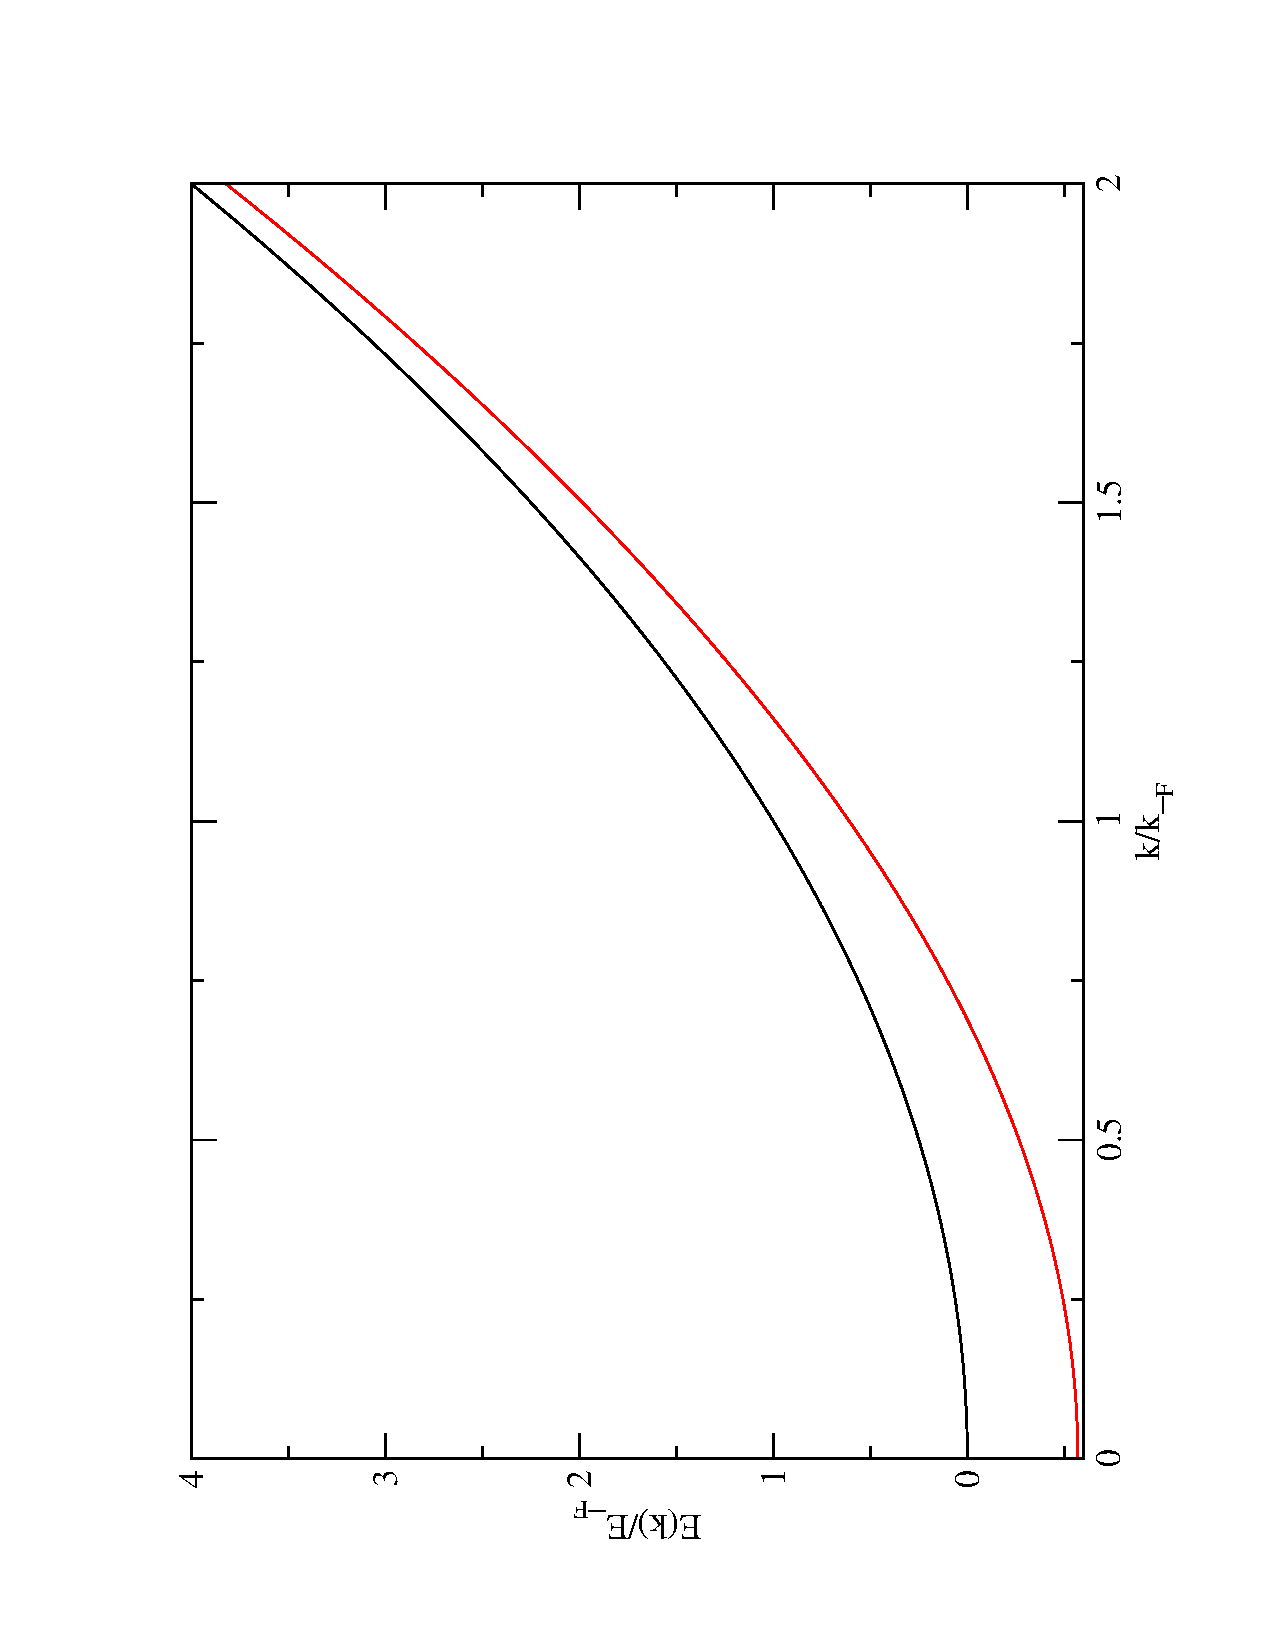
\includegraphics[angle=-90,origin=c,scale=0.2,trim={1cm 0 1cm 0},clip]{grafy/screening_erg} }}%
    \subfloat{{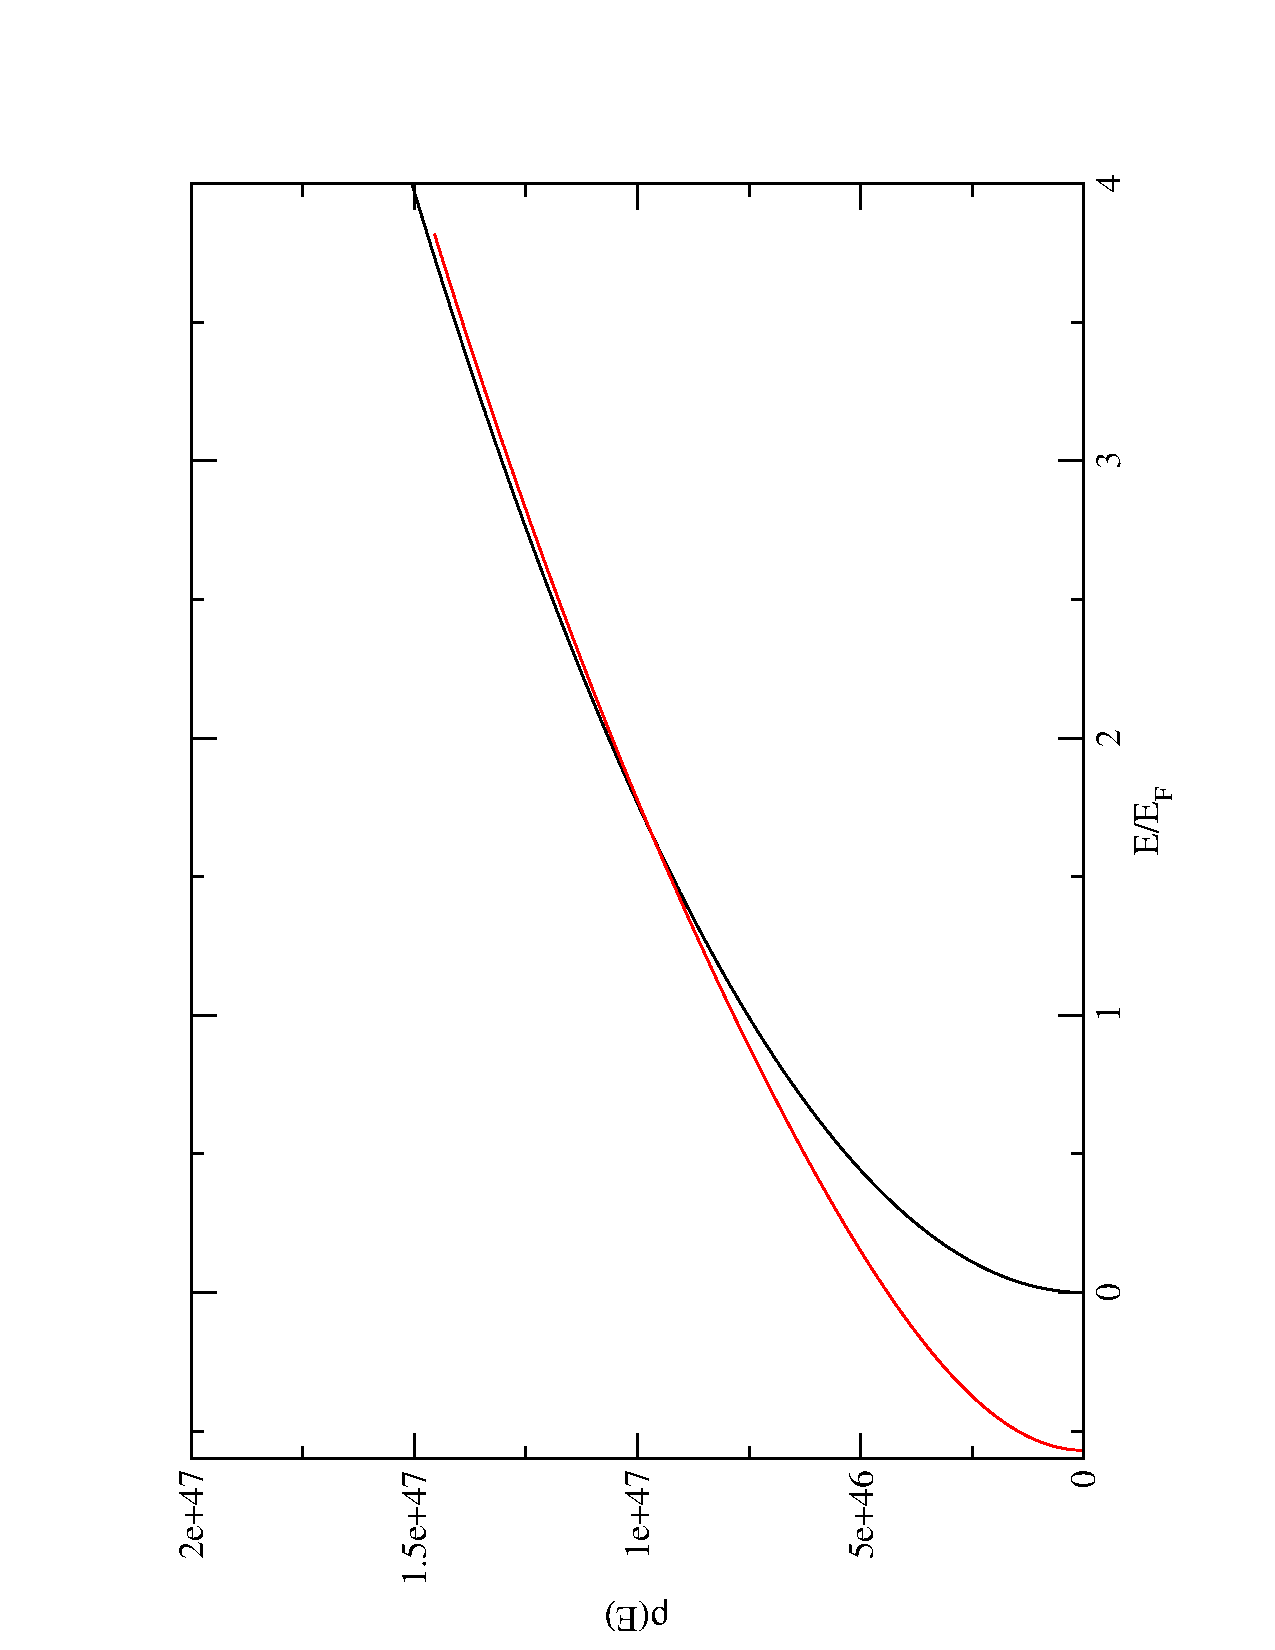
\includegraphics[angle=-90,origin=c,scale=0.2,trim={1cm 0 1cm 0},clip]{grafy/screening_dos} }}%
    \vspace{-10mm}
    \small
    \normalsize
    \label{fig:example}%
\end{figure}
Panel vľavo: červená čiara ukazuje disperzný zákon podľa rovnice (14), čierna čiara ukazuje parabolický disperzný zákon neinteragujúcich elektrónov. Panel vpravo: červená a čierna čiara zobrazujú zodpovedajúce hustoty stavov.
\end{frame}
\begin{frame}

\note{Elektrón v disorderovanom kove bez e-e interakcie je popísaný Sch. R. \eqref{eq:schr_dis}.  Započítaním e-e interakcie v modeli \emph{želé} dostaneme Fockovu rovnicu \eqref{eq:fock_dis}.  Problém \eqref{eq:fock_dis} riešime v prvom ráde poruchovej teórie. $\phi_m(\vr) \simeq \phi_m^{(0)}(\vr)$. Problém  \eqref{eq:fock_dis} je pre jeden konkrétny disorder. Náš výsledok je stredovaný cez súbor mikroskopicky rôznych ale makroskopicky rovnakých disrderov. Pre stredný disorder dostaneme  \eqref{eq:erg_meandis}.
Poruchové riešenie
$\phi_m(\vr) \simeq \phi_m^{(0)}(\vr)$ môžeme na rovnicu  \eqref{eq:fock_dis} aplikovať len vtedy,
keď je interakcia $V(\vr-\vrp)$ slabá v porovnaní s interakciou s disorderom.
To je pravda pre medzielektrónové vzdialenosti $|\vr-\vrp| \gtrsim l$, pretože na vzdialenostiach $>l$ sa už interakcia s disorderom uplatňuje,
zatiaľčo interakcia $V(\vr-\vrp)$ je exponenciálne zatienená už na vzdialenosti $|\vr-\vrp| \simeq k_s^{-1} \simeq k_F^{-1} \ll l$.
Keď však dva elektróny navzájom interagujú vo vzdialenosti $|\vr-\vrp| \lesssim l$, interakcia s disorderom sa nestihne uplatniť.
To znamená že interakcia $V(\vr-\vrp)$ na vzdialenostich $|\vr-\vrp| \lesssim l$ nie je v porovnaní s disorderom slabá porucha.
Intuitívne je jasné, že správny poruchový ansatz v tomto prípade musí byť rovinná vlna
$\phi_m(\vr) \simeq \frac{1}{\sqrt V}e^{i\vk_m\cdot\vr}$, ktorá je správnym riešením Fockovej rovnice v modeli želé bez disorderu.
}

\frametitle{Elektrón-elektrónová interakcia v kove s disorderom : Jav Altshulera - Aronovova}
\begin{itemize}
\item Elektrón v disorderovanom kove bez e-e interakcie je popísaný Sch. R.
\begin{equation}
\label{eq:schr_dis}
\bigl(-\frac{\hbar^2}{2m}\laplace + V_{dis}(\vr)\bigr)\phi_m^{(0)}(\vr)=\E_m\phi_m^{(0)}(\vr) \text{,}
\end{equation}
\item Započítaním e-e interakcie v modeli \emph{želé} dostaneme Fockovu rovnicu
\small
\begin{equation}
 \label{eq:fock_dis}
 \bigl(-\frac{\hbar^2}{2m}\laplace + V_{dis}(\vr) \bigr)\phi_m(\vr)-\sum_{\forall m'} \int d\vrp \phi^*_{m'}(\vr)\phi_{m}(\vrp)V(\vr-\vrp)\phi_{m'}(\vr)=E_m\phi_m(\vr) \text{.}
\end{equation}
\normalsize
\item Problém \eqref{eq:fock_dis} riešime v prvom ráde poruchovej teórie. $\phi_m(\vr) \simeq \phi_m^{(0)}(\vr)$
\item Pre stredný disorder dostaneme 
\small
\begin{equation}
\label{eq:erg_meandis}
 \overline{E_m}=\overline{\E_m}-\sum_{\forall m'} \frac{1}{(2\pi)^{3}} \int d\vq\ V(q) \overline{|\bra{\phi_m}e^{i\vq\cdot\vr}\ket{\phi_{m'}}|^2} \text{.}
\end{equation}
\normalsize
\item poruchová teória platí len pre $q<q_{max}=\frac{A}{l}$ kde $A\simeq 1$ a $l$ je stredná voľná dráha elektrónu. Pre $q>q_{max}$ aproximujeme $\phi_m(\vr)$ rovinnými vlnami.
\end{itemize}
\end{frame}
\begin{frame}
\note
{
Pre výpočet energie nám stačí maticový element \eqref{eq:aa_matrix_element}. Počítame difúznou aproximáciou, podobne ako AA. 
 Difúzna aproximácia spočíva v postulovaní rovnice \eqref{eq:aa_postulate}, teda že elektrón sa správa ako brownowská častica.
  Vlnovú funkciu častice z rovnice \eqref{eq:aa_postulate} rozvinieme do stacionárnych stavov $\phi_m(\vr)$.
  Difúzna aproximácia platí len za predpokladu $|\E_m-\E_{m'}|\ll\hbar / \tau$. Z difúznej aproximácie vieme dostať maticový element, ktorý dosadíme  do rovnice pre energiu \eqref{eq:erg_meandis}
}

\begin{itemize}
\item Potrebujeme vypočítať maticový element
\begin{equation}
\label{eq:aa_matrix_element}
\overline{| M_{mm'}|^2} =\overline{|\bra{\phi_m}e^{i\vq\cdot\vr}\ket{\phi_{m'}}|^2} \text{.}
\end{equation}
\item Altshuler a Aronov použili difúznu aproximáciu, ktorá spočíva v postulovaní rovnice
\begin{equation}
 \label{eq:aa_postulate}
 \overline{\psi^*(\vr,t)\psi(\vr,t)}=\frac{1}{(4\pi Dt)^{3/2}}e^{-\frac{|\vr-\vr_0|^2}{4Dt}} \text{,}
\end{equation}
\item vlnovú funkciu častice z rovnice \eqref{eq:aa_postulate} rozvinieme do stacionárnych stavov $\phi_m(\vr)$
\begin{equation}
 \label{eq:aa_psi_sum}
 \psi(\vr,t)=\frac{\sqrt{V}}{\sqrt{N}}\sum_m \phi_m^*(\vr_0)\phi_m(\vr)e^{-i\frac{\E_m}{\hbar}t} \text{,}
\end{equation}
\item Difúzna aproximácia platí len za predpokladu $|\E_m-\E_{m'}|\ll\hbar / \tau$
\item Z difúznej aproximácie sa dá pre maticový element odvodiť výsledok
\begin{equation}
 \label{eq:aa_matrix_element_final}
 \overline{|M_{\E, \E'}|^2}=\frac{1}{\pi \rho(\E')} \frac{\hbar D q^2}{(\E-\E')^2+(\hbar Dq^2)^2}\text{,}
\end{equation}
\end{itemize}
\end{frame}
\begin{frame}
\note{
rovnicu \eqref{eq:erg_meandis modif}  zapíšeme v tvare  $\overline{E(\E})=\overline\E+E_{self}(\E)$. 
 derivujeme podľa počtu stavov a dostaneme   otočením oboch strán dostaneme hustotu stavov, ktorú počítame ako Taylorov rozvoj do prvého rádu
\eqref{eq:der}. Otočením oboch strán dostaneme hustotu stavov, ktorú počítame ako Taylorov rozvoj do prvého rádu. Dosadením self energie dostaneme Altschuler-Aronovov výsledok \eqref{eq:aa_dos3 fin}, kde vidíme potlačenie hustoty v okolí Fermiho energie.
}

\begin{itemize}
\item rovnicu (17)  zapíšeme v tvare  
\begin{equation}
E(\E)=\E+E_{self}(\E)
\end{equation}
 kde 
\begin{equation}
 \label{eq:aa_self_energy}
 E_{self}=-\int_{0}^{\E_F}d\E' \int \frac{d\vq}{8\pi^4}V(q)\frac{\hbar D q^2}{(\hbar D q^2)+(\E-\E')}\text{,}
\end{equation}

\item Rovnicu (22) derivujeme podľa počtu stavov a dostaneme 
\begin{equation}
\label{eq:der}
  \frac{d E(\E)}{dn}=\frac{d\E}{dn}+\frac{dE_{self}(\E)}{dn}=\frac{d\E}{dn}+\frac{dE_{self}(\E)}{d\E}\frac{d\E}{dn}=\frac{d\E}{dn}(1+\frac{dE_{self}(\E)}{d\E}) \text{.}
\end{equation}
\item otočením oboch strán poslednej rovnice dostaneme hustotu stavov
\begin{equation}
 \label{eq:aa_dos2}
 \rho(\E) \simeq \rho_0(\E)[1-\frac{dE_{self}(\E)}{d\E}] \simeq \rho_0(\E_F)[1-\frac{dE_{self}(\E)}{d\E}] \text{.}
\end{equation}
\item Dosadením self energie dostaneme Altshulerov-Aronovov výsledok
\begin{equation}
 \label{eq:aa_dos3 fin}
 \rho(\E)=\rho_0(\E_F) - \frac{q_{max}}{2\pi^3 \hbar D}
 +    \frac{1}{2\pi^2 (2\hbar D)^{3/2}}  \ \sqrt{|\E-\E_F|}  \text{.}
\end{equation}
\end{itemize}
\end{frame}
\begin{frame}
\note{
Hustotu stavov meriame podľa obrázka. Vľavo máme čistý kov, ktorého hustotu stavov poznáme. Vpravo máme kov s disorderom. Oddelené sú tenkou vrstvou izolantu = barieru. 
Elektróny tunelujú cez barieru ako popisuje pásový diagram na obrázku. Meraním diferenciálnej vodivosti sústavy vieme určiť hustotu stavov. 

}
\frametitle{Meranie hustoty stavov v kove s disorderom metódou tunelovej spektroskopie}
\vspace{-15mm}
\begin{figure}%
    \centering
    \subfloat{{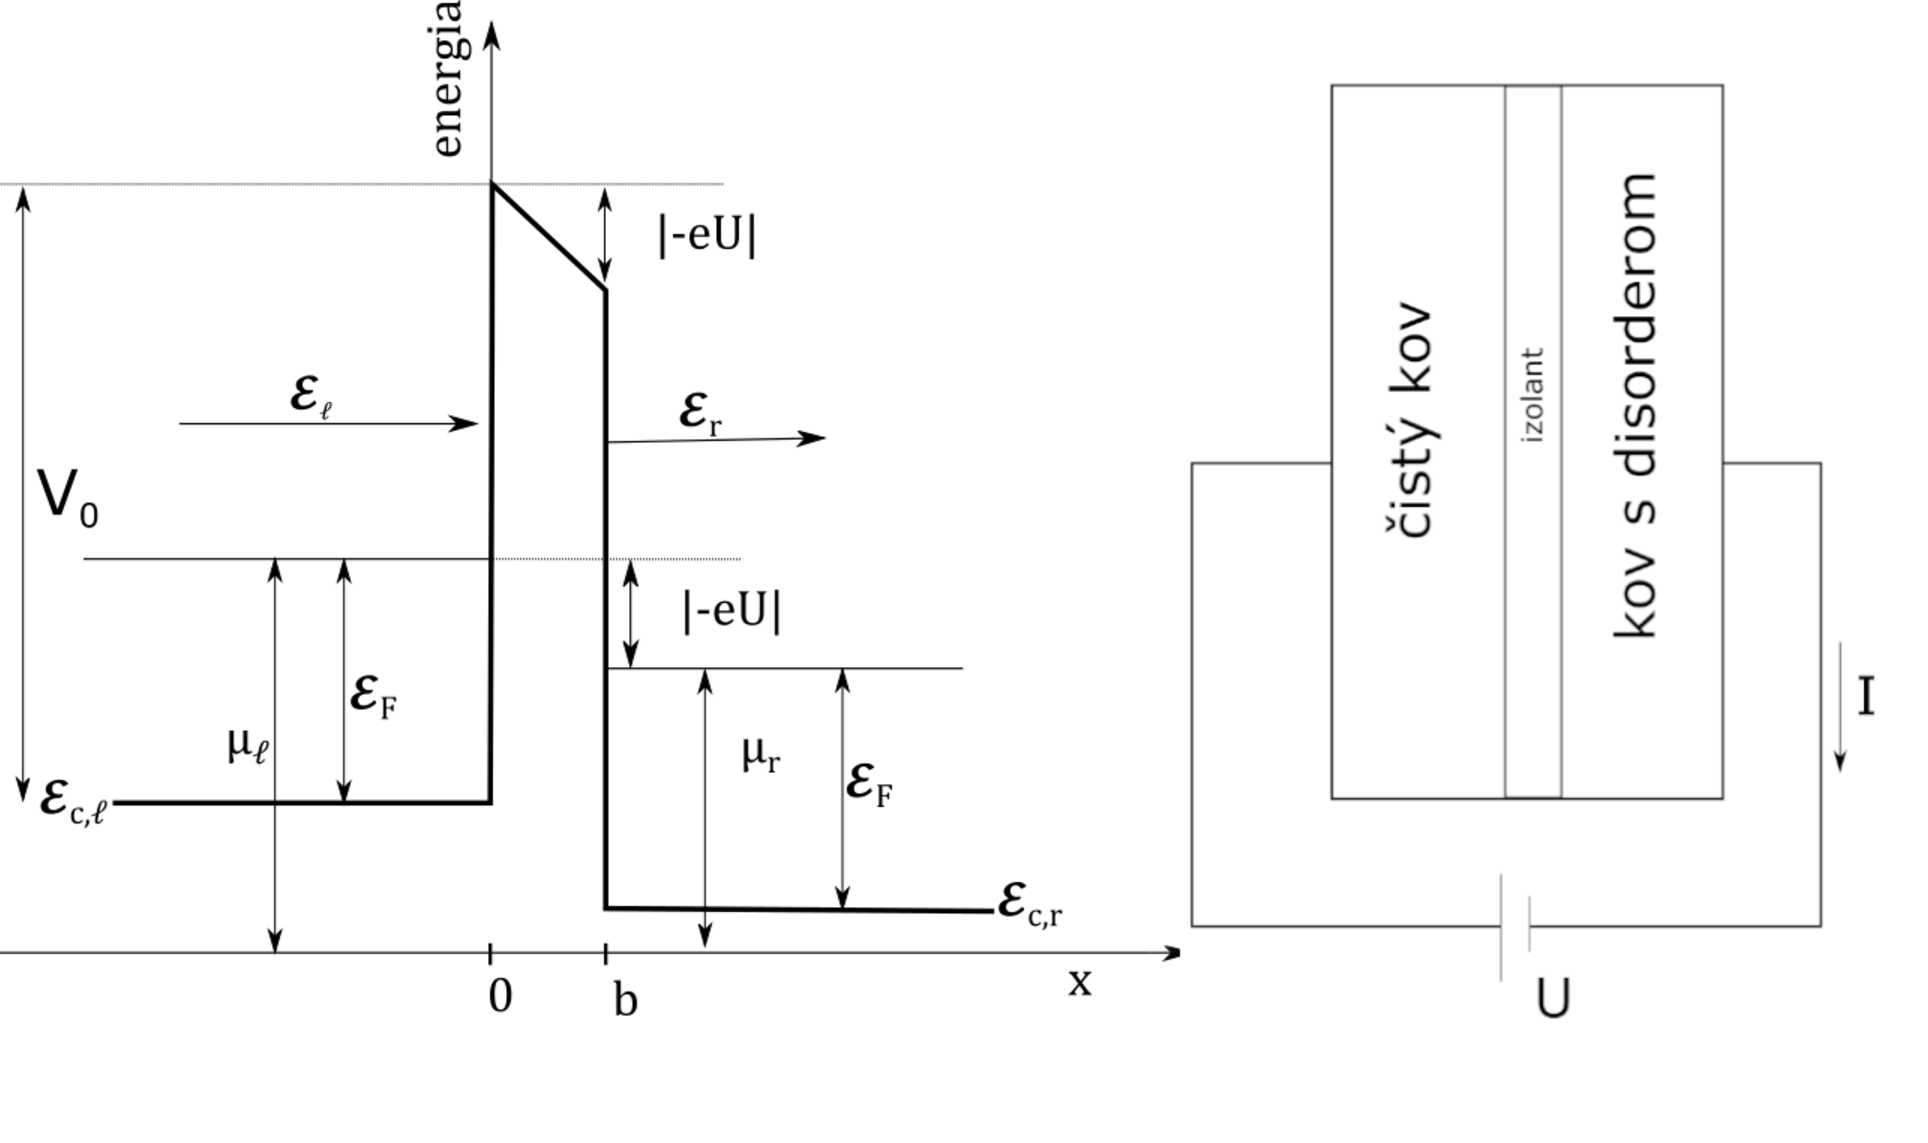
\includegraphics[scale=0.25]{grafy/fuck_beamer} }}%
    \vspace{-10mm}
    \label{fig:example}%
\end{figure}
\small
Hustotu stavov určíme meraním diferenciálnej vodivosti dvoch kovov oddelených tenkou vrstvou izolantu, ako je ukázané na obrázku. 
Dá sa ukázať, že pre diferenciálnu vodivosť platí vzťah
$G(U)=e^2\frac{4\pi|t|^2}{\hbar}\rho_l(\E_F)\rho_r(\E=\E_F-eU)$, kde $\rho_r(\E)$ je hľadaná hustota stavov, ktorú chceme odmerať.  
\normalsize
 \end{frame}
\begin{frame}
\note{
Výsledky merania hustoty stavov tunelovou spektroskopiou pre rôzne kovy
V blízkom okolí Fermiho energie všetky ukázané spektrá vykazujú Altshuler-Aronovov jav pokles úmerný odmocnine. Ďaleko od Fermiho energie už Altshuler-Aronovova závislosť
 očividne neplatí a pre dostatočne veľké hodnoty vidno, že hustota stavov klesá k $\rho_0$ zhora.
}
\vspace{-10mm}
\begin{figure}%
    \centering
    \subfloat{{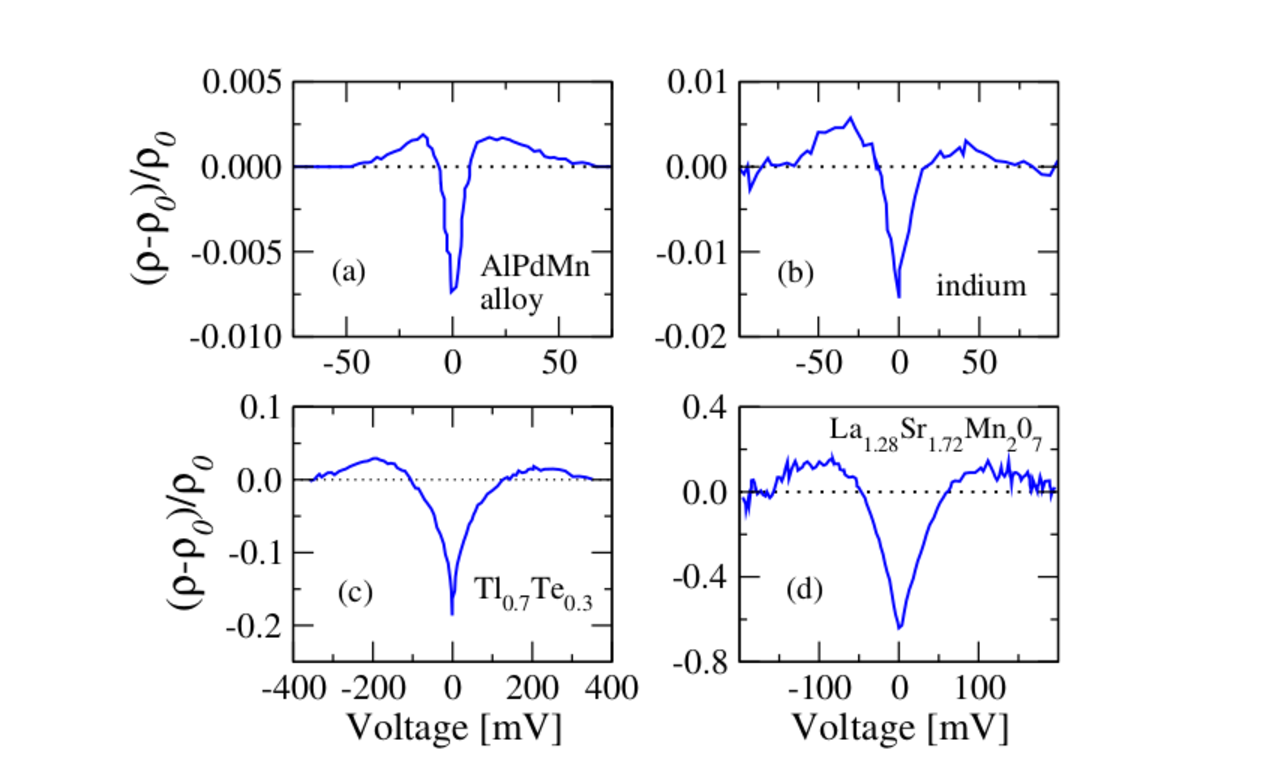
\includegraphics[scale=0.5]{grafy/B2} }}%
    %\subfloat{{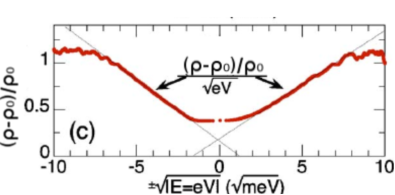
\includegraphics[scale=0.4]{grafy/dos-altschuler} }}%
    \label{fig:example}%
\end{figure}
\small
Výsledky merania hustoty stavov tunelovou spektroskopiou pre rôzne kovy
V blízkom okolí Fermiho energie všetky ukázané spektrá vykazujú Altshuler-Aronovov jav $\rho(|\E- \E_F|) \propto \sqrt{|\E- \E_F|}$. Ďaleko od Fermiho energie už Altshuler-Aronovova závislosť
$\rho(|\E- \E_F|) \propto \sqrt{|\E- \E_F|}$ očividne neplatí a pre dostatočne veľké hodnoty $|\E - \E_F|$ vidno, že $\rho(|\E- \E_F|)$ s rastúcim $|\E - \E_F|$ klesá k $\rho_0$ zhora.
\normalsize
\end{frame}
\begin{frame}
\note{
Altschuler-Aronovov výsledok platí len pre energie $< \hbar/\tau$.  Z AA výsledku vidno že hustota stavov sa pretne s neporušenou pre $|\E-\E_F| =  U_{co}$
tzv. korelačná energia. Pre energie oveľa väčšie ako kondenzačná experiment ukazuje, že stavy vytlačené z oblasti pod kondenzačnou energiou majú tendenciu sa nakopiť tesne
nad energiou ňou v oblasti veľkosti dva a až tri krát kondenzačná energuia, čo AA vôbec nepopisuje. Teóriu sa pokúsime rozšíriť do oblastí nad korelačnú energiu.
}
\frametitle{Altshuler - Aronovov jav, rozšírenie teórie na energie $|\E - \E_F| \gtrsim \hbar/\tau$}
\begin{itemize}
\item Altschuler-Aronovov výsledok platí len pre energie $|\E - \E_F| < \hbar/\tau$
\item Z AA výsledku vidno že $\rho(\E) = \rho_0$ pre $|\E-\E_F| =  U_{co}$, kde
\begin{equation}
\label{eq:aa_U co korelenergia}
 U_{co} = \frac{8}{3\pi^{2}} q_{max}^2 l^2 \frac{\hbar}{\tau} 
\end{equation}

je korelačná energia
\item Pre $|\E-\E_F| \gtrsim  U_{co}$ experiment ukazuje, že stavy vytlačené z oblasti $|\E-\E_F| \lesssim  U_{co}$ majú tendenciu sa nakopiť tesne
nad energiou $|\E-\E_F| =  U_{co}$ v oblasti veľkosti dva a až tri krát $U_{co}$.
\item Pokiaľ je nám známe,tak tento experimentálny výsledok (najmä fakt, že  pre $|E-E_F| > U_{co}$ hodnota $\rho(\E)$ hodnotu $\rho_0$
najprv prevýši a až potom k nej konverguje zhora) nemá oporu v dostupných teóriach.
\item preto sa pokúsime teóriu rozšíriť do oblasti  $|\E-\E_F| \gtrsim U_{co}$
\end{itemize}
\end{frame}

\begin{frame}
\note{
 Vychádzame z rovnice \eqref{eq:erg_meandis nex}. 
 Pre $q > q_{max} \simeq 1/l$ je treba vlnové funkcie $\phi_m(\vr)$ aproximovať rovinnými vlnami $\frac{1}{\sqrt V}e^{i\vk_m\cdot\vr}$, zatiaľčo pre $q < q_{max}$ treba
$\phi_m(\vr)$ považovať za vlnové funkcie elektrónov interagujúcich len s disorderom. 
}
\begin{itemize}
\item vychádzame z Fockovej rovnice
\begin{equation}
\label{eq:erg_meandis nex}
 \overline{E_m}=\overline{\E_m}-\sum_{\forall m'} \frac{1}{(2\pi)^{3}} \int d\vq\ V(q) \overline{|\bra{\phi_m}e^{i\vq\cdot\vr}\ket{\phi_{m'}}|^2} \text{.}
\end{equation}
kde $V(q) = e^2/\epsilon_0(q^2+k_s^2)$.
\item pre $q > q_{max} \simeq 1/l$ aproximujeme vlnové funkcie $\phi_m(\vr)$ rovinnými vlnami $\frac{1}{\sqrt V}e^{i\vk_m\cdot\vr}$, zatiaľčo pre $q < q_{max}$ aproximujeme
$\phi_m(\vr)$ vlnovými funkciami elektrónov interagujúcich len s disorderom:
\begin{equation}\label{eq:erg_meandis nex nex}
\begin{split}
 \overline{E_m}= &\frac{\hbar^2 k_m^2}{2m} - \sum_{\forall m'} \frac{1}{(2\pi)^{3}} \int_{|\vq| < q_{max}} d\vq\ V(q) \overline{|\bra{\phi_m}e^{i\vq\cdot\vr}\ket{\phi_{m'}}|^2}  \\
    &  - \sum_{\forall m'} \frac{1}{(2\pi)^{3}} \int_{|\vq| > q_{max}} d\vq\ V(q) |\bra{k_m}e^{i\vq\cdot\vr}\ket{k_{m'}}|^2 \text{.}
\end{split}
\end{equation}
kde $\ket{k_{m}}= \frac{1}{\sqrt V}e^{i\vk_m\cdot\vr}$
\end{itemize}
\end{frame}
\begin{frame}
\note{

 Rovnicu prepíšeme do tvaru \eqref{eq:erg_meandis nex prepis skratka}. \\
 je energia voľného elektrónu interagujúceho s ostatnými cez tienenú Fockovu e-e interakciu\\
 je Altschuler Aronovova self eneria, ktorú AA počítali difúznou aproximáciou \\
 je self-energia pochádzajúca z Fockovho príspevku od rovinných vĺn, túto self energiu aa nezapocitali
 
}

\begin{itemize}
\item Rovnicu \eqref{eq:erg_meandis nex nex} prepíšeme do tvaru
\begin{equation}\label{eq:erg_meandis nex prepis skratka}
 \overline{E_m} \ \ = \ \ \E_m + E_{self}^{AA}(m) - E_{self}^{free}(m)  \text{,}
\end{equation}
kde
\begin{equation}\label{eq:erg_volna castica s ee}
\E_m = \frac{\hbar^2 k_m^2}{2m} - \sum_{\forall m'} \frac{1}{(2\pi)^{3}} \int d\vq\ V(q) |\bra{k_m}e^{ivq\cdot\vr}\ket{k_{m'}}|^2  \text{}
\end{equation}
je energia voľného elektrónu interagujúceho s ostatnými cez tienenú Fockovu e-e interakciu,
\begin{equation}\label{eq:erg_self AA}
 E_{self}^{AA}(m) \ \ = \ \  -\sum_{\forall m'} \frac{1}{(2\pi)^{3}} \int_{|\vq| < q_{max}} d\vq\ V(q) \overline{|\bra{\phi_m}e^{i\vq\cdot\vr}\ket{\phi_{m'}}|^2}  \text{}
\end{equation}
je Altshulerova-Aronovova self energia
\begin{equation}\label{eq:erg_self free}
 E_{self}^{free}(m) \ \ =  \ \  - \sum_{\forall m'} \frac{1}{(2\pi)^{3}} \int_{|\vq| < q_{max}} d\vq\ V(q) |\bra{k_m}e^{i\vq\cdot\vr}\ket{k_{m'}}|^2\text{,}
\end{equation}
je self-energia pochádzajúca z Fockovho príspevku od rovinných vĺn
\end{itemize}
\end{frame}
\begin{frame}
\note{
Počítame \eqref{eq:erg_self AA}. Altshuler a Aronov počítali v difúznej aproximácii, my zvolíme iný postup.
 vlnové funkcie $\phi_m(\vr)$ rozvinieme do úplneho systému rovinných vĺn. Využijeme ortogonalitu, čo nám umožní sumovať cez Kroneckerove symboly.

}
\begin{itemize}
\item Počítame \eqref{eq:erg_self AA}. Altshuler a Aronov počítali v difúznej aproximácii, my zvolíme iný postup.
\item vlnové funkcie $\phi_m(\vr)$ rozvinieme do úplneho systému rovinných vĺn $\phi_m(\vr) = \frac{1}{\sqrt{\Omega}}\sum_{\vk}c_{\vk}^me^{i\vk\vr}$. 
\tiny
\begin{multline}
E_{self}^{AA}(m)=  - \frac{1}{(2\pi)^3\Omega^2}     \\
\times  \int_{|\vq| < q_{max}} d\vq\ V(\vq)\overline{ \sum_{m'} \sum_{\vk_1} \sum_{\vk_3}\int d\vr c^{m*}_{\vk_1}c^{m'}_{\vk_3}e^{i\vq\cdot q\vr}e^{i\vk_1\cdot \vr}e^{-i\vk_3\cdot \vr} \sum_{\vk_2}\sum_{\vk_4} \int d\vrp c^{m'*}_{\vk_4}c^{m}_{\vk_2}e^{-i\vq\cdot \vrp}e^{-i\vk_4\cdot \vrp}e^{i\vk_2\cdot \vrp}} \text{.}
\end{multline}
\normalsize
\item Využijeme vzťahy
\begin{equation}
\frac{1}{\Omega}\ \int d\vr\ e^{i(\vk_1+\vq-\vk_3)\vr}=\delta_{\vk_3,\vk_1+\vq}
\  \   \  \text{,}
\ \
\frac{1}{\Omega} \ \int d\vrp e^{i(\vk_2-\vq-\vk_4)\vrp}=\delta_{\vk_2,\vk_4+\vq}
\ \ \  \text{.}
\end{equation}

\end{itemize}
\end{frame}

\begin{frame}
\note{
Po vysumovaní s pomocou Kroneckerovych symbolov dostaneme \eqref{eq:self aa}\\
Začíname robiť aproximácie. Stavy $m$ a $m'$ považujeme za nekorelované. \\
Navyše predpokladáme, že aj stavy $\vk$ a $\vkp$ sú nekorelované.\\
rovnicu \eqref{eq:self aa} pomocou aproximáciii zjednodušíme na \eqref{eq:05energy2}\\
\small
Nekorelovane sú preto, lebo ccka sú komplexné cisla.  2 stavy sa lisia iba o nahodnu fazu, ktoru vyberam nezavisle.
Preto su nekorelovane aj k aj m.
\normalsize

}
\begin{itemize}
\item Po vysumovaní dostaneme
\begin{align}
\label{eq:self aa}
E_{self}^{AA}(m)= - \frac{1}{(2\pi)^3}\int_{|\vq| < q_{max}} d\vq\ V(\vq) \sum_{m'}\sum_{\vk}\sum_{\vkp}\overline{c^{*m}_{\vk+\vq}c^{m}_{\vk\ '+\vq}c^{*m'}_{\vk\ '}c^{m'}_{\vk}}\text{.}
\end{align}
\item Začíname robiť aproximácie. Stavy $m$ a $m'$ považujeme za nekorelované. 
\item Navyše predpokladáme, že aj stavy $\vk$ a $\vkp$ sú nekorelované.
\item rovnicu \eqref{eq:self aa} pomocou aproximáciii zjednodušíme na
\begin{align}
\label{eq:05energy2}
E_{self}^{AA}(m)= - \frac{1}{(2\pi)^3} \int_{|\vq| < q_{max}} d\vq\ V(\vq) \sum_{m'}\sum_{\vk} \overline{c^{m*}_{\vk+\vq}c^{m}_{\vk+\vq}}\ \overline{c^{*m'}_{\vk}c^{m'}_{\vk}} \text{.}
\end{align}
\end{itemize}
\end{frame}
\begin{frame}
\note{
Využijeme Thoulessov Ansatz \eqref{eq:05thouless}.\\
Thouless [22] použil aproximáciu \eqref{eq:05thouless} pri opise vlnových funkcií neusporiadaného elektrónového systému v kvantovej vodivosti Kuba - Greenwooda
Ukázal, že aproximácia \eqref{eq:05thouless} spôsobí, že kvantová vodivosť Kuba - Greenwooda prejde na klasickú Drudeho vodivosť
Naše odvodenie self-energie  $E_{self}^{AA}(m)$sa opiera o tie isté aproximácie, ako použil Thouless
}
\begin{itemize}
\item Využijeme Thoulessov Ansatz - tzv. self konzistentnú Bornovu aproximáciu
\begin{align}
\label{eq:05thouless}
\overline{c^{m*}_{\vk}c^{m}_{\vk}}=\frac{1}{\pi \rho(\epsilon_m)}\lorenz{\epsilon_m} \text{,}
\end{align}
kde $\tau$ je semiklasický elektrónový zrážkový čas pre rozptyl na prímesnom disorderi. 
\item Thouless [22] použil aproximáciu \eqref{eq:05thouless} pri opise vlnových funkcií neusporiadaného elektrónového systému v kvantovej vodivosti Kuba - Greenwooda
\item Ukázal, že aproximácia \eqref{eq:05thouless} spôsobí, že kvantová vodivosť Kuba - Greenwooda prejde na klasickú Drudeho vodivosť
\item Naše odvodenie self-energie  $E_{self}^{AA}(m)$sa opiera o tie isté aproximácie, ako použil Thouless
\end{itemize}
\end{frame}
\begin{frame}
\note{
do rovnice pre $E_{self}^{AA}(m)$ dosadíme Thoulessov ansatz a prejdeme od sumy k integrálu\\
kde sme zaviedli pomocné označenia.\\
Hustota stavov $\rho(\epsilon_m')$ sa vykráti, ale ostatné nie. Napriek tomu ich kvôli jednoduchosti približne vykrátime.\\
po prechode do sférických súradníc pri integrovaní cez $d\vq$ dostávame \eqref{eq:05energy5} \\
Integrál cez $d\phi$ je $2\pi$, integrály cez $d\epsilon_m$ a $d\theta$ vieme vypočítať analyticky, a zvyšné dva budeme rátať numericky



}

\begin{itemize}
\item do rovnice pre $E_{self}^{AA}(m)$ dosadíme Thoulessov ansatz a prejdeme od sumy k integrálu
\tiny
\begin{multline}
E_{self}^{AA}(\epsilon_m)= - \frac{1}{(2\pi)^3} \\
\int_{|\vq| < q_{max}} d\vq\ V(\vq)\int d\epsilon_k \rho(\epsilon_k) \int_0^{\epsilon_F} d\epsilon_{m'} \rho(\epsilon_{m'})\frac{1}{\pi\rho(\epsilon_m)}\frac{\epsilon_\tau}{(\epsilon_m-\epsilon_k)^2+
\epsilon_\tau^2}\frac{1}{\pi\rho(\epsilon_{m'})}\frac{\epsilon_\tau}{(\epsilon_{m'}-\epsilon_{|\vk+\vq|})^2+\epsilon_\tau^2} \text{.}
\end{multline}
\normalsize
kde $\epsilon_\tau \equiv \frac{\hbar}{2\tau}$ a $\epsilon_{|\vk+\vq|} \equiv\frac{\hbar^2|\vk+\vq\ |^2}{2m}$.
\item Hustota stavov $\rho(\epsilon_m')$ sa vykráti, ale hustoty stavov $\rho(\epsilon_{k})$ a $\rho(\epsilon_m)$ nie. Napriek tomu ich kvôli jednoduchosti približne vykrátime.
\item po prechode do sférických súradníc pri integrovaní cez $d\vq$ dostávame
\small
\begin{align}
\label{eq:05energy5}
\notag
E_{self}^{AA}(\epsilon_m)= - \frac{1}{(2\pi)^3}\frac{1}{\pi^2}\int_0^{2\pi}d\phi \int_0^\pi d\theta \sin\theta \ \int_0^{q_{max}} dq\ q^2 V(q)\\
\int_0^{\E_F} d\epsilon_{m'} \int_0^{\infty} d \epsilon_k \frac{\epsilon_\tau}{(\epsilon_m-\epsilon_k)^2+\epsilon_\tau^2}\frac{\epsilon_\tau}{(\epsilon_{k}+\epsilon_{q}+2\sqrt{\epsilon_{k}\epsilon_{q}}\cos(\theta)-\epsilon_{m'})^2+\epsilon_\tau^2} \text{.}
\end{align}
\normalsize
\item Integrál cez $d\phi$ je $2\pi$, integrály cez $d\epsilon_m$ a $d\theta$ vieme vypočítať analyticky, a zvyšné dva budeme rátať numericky
\end{itemize}
\end{frame}
\begin{frame}
\note{
po formálnom vystredovaní \eqref{eq:erg_meandis nex prepis skratka}  rovnica prejde na tvar \eqref{eq:energia} \\
rovnicu \eqref{eq:energia} derivujeme podľa počtu stavov a prevrátime. Následne po Taylorovom rozvoji a úpravách dostaneme \eqref{eq:erg_meandis nex prepis skratka7}.
kde sme urobili aproximáciu $\frac{d\epsilon}{d\E} \simeq 1$  čo znamená aj aproximáciu $\epsilon \simeq \E$.
hustotu stavov plotujeme v tvare relatívnej odchýlky,v tomto tvare prepíšeme aj pôvodný vzťah Altschulera a Aronova. V tomto tvare sa hustota stavov meria v experimentoch.

}

\begin{itemize}
\item po vystredovaní rovnice (30) $\frac{1}{\rho(\epsilon)}\sum_{\forall m} \delta(\epsilon-\epsilon_{m})$
rovnica (30) prejde na tvar
\begin{equation}
\label{eq:energia}
 \overline{E} \ \ = \ \ \E(\epsilon) + E_{self}^{AA}(\epsilon) - E_{self}^{free}(\epsilon)  \text{.}
\end{equation}
\item dostaneme hustotu stavov
 \begin{equation}\label{eq:erg_meandis nex prepis skratka7}
\rho(\E) \ \ = \rho_0(\E) [1 - \frac{dE_{self}^{AA}(\E)}{d\E} + \frac{dE_{self}^{free}(\E)}{d\E}] \text{,}
\end{equation}

\item hustotu stavov plotujeme v tvare relatívnej odchýlky
\begin{equation}\label{eq:erg_hustota stavov relat}
\frac{\rho(\E) - \rho_0(\E)}{\rho_0(\E)} = - \frac{dE_{self}^{AA}(\E)}{d\E} + \frac{dE_{self}^{free}(\E)}{d\E} \text{,}
\end{equation}
\item v tomto tvare prepíšeme aj pôvodný vzťah Altschulera a Aronova
\begin{equation}\label{eq:erg_hustota stavov relat povodny}
\frac{\rho(\E) - \rho_0(\E)}{\rho_0(\E)} = - \frac{e^{2}}{\epsilon_0 k_s^{2}}\ \  \frac{q_{max}}{2\pi^3 \hbar D}
 +  \frac{e^{2}}{\epsilon_0 k_s^{2}} \ \ \frac{1}{2\pi^2 (2\hbar D)^{3/2}}  \ \sqrt{|\E-\E_F|} \text{,}
\end{equation}
\end{itemize}
\end{frame}

\begin{frame}
\note{
Panel (a): Krivka ukázaná červenou farbou je pôvodná závislosť Altshulera - Aronova \eqref{eq:erg_hustota stavov relat povodny}.
krivka ukázaná modrou farbou ukazuje prvý člen numerického výpočtu \eqref{eq:erg_hustota stavov relat} . Panel (c) ukazuje obidva grafy z panelu (a) este raz, avšak "zošité" približne v energii  $|\E-\E_F| = U_{co}$. Panel (b) ukazuje druhý člen  \eqref{eq:erg_hustota stavov relat} . Panel (d) ukazuje celkovú závislosť $\frac{\rho(\E) - \rho_0(\E)}{\rho_0(\E)}$, získanú sčítaním grafov v paneloch (b) a (c).
}
\frametitle{Výsledky a ich diskusia}
\begin{columns}[c]

\begin{column}{.5\textwidth}
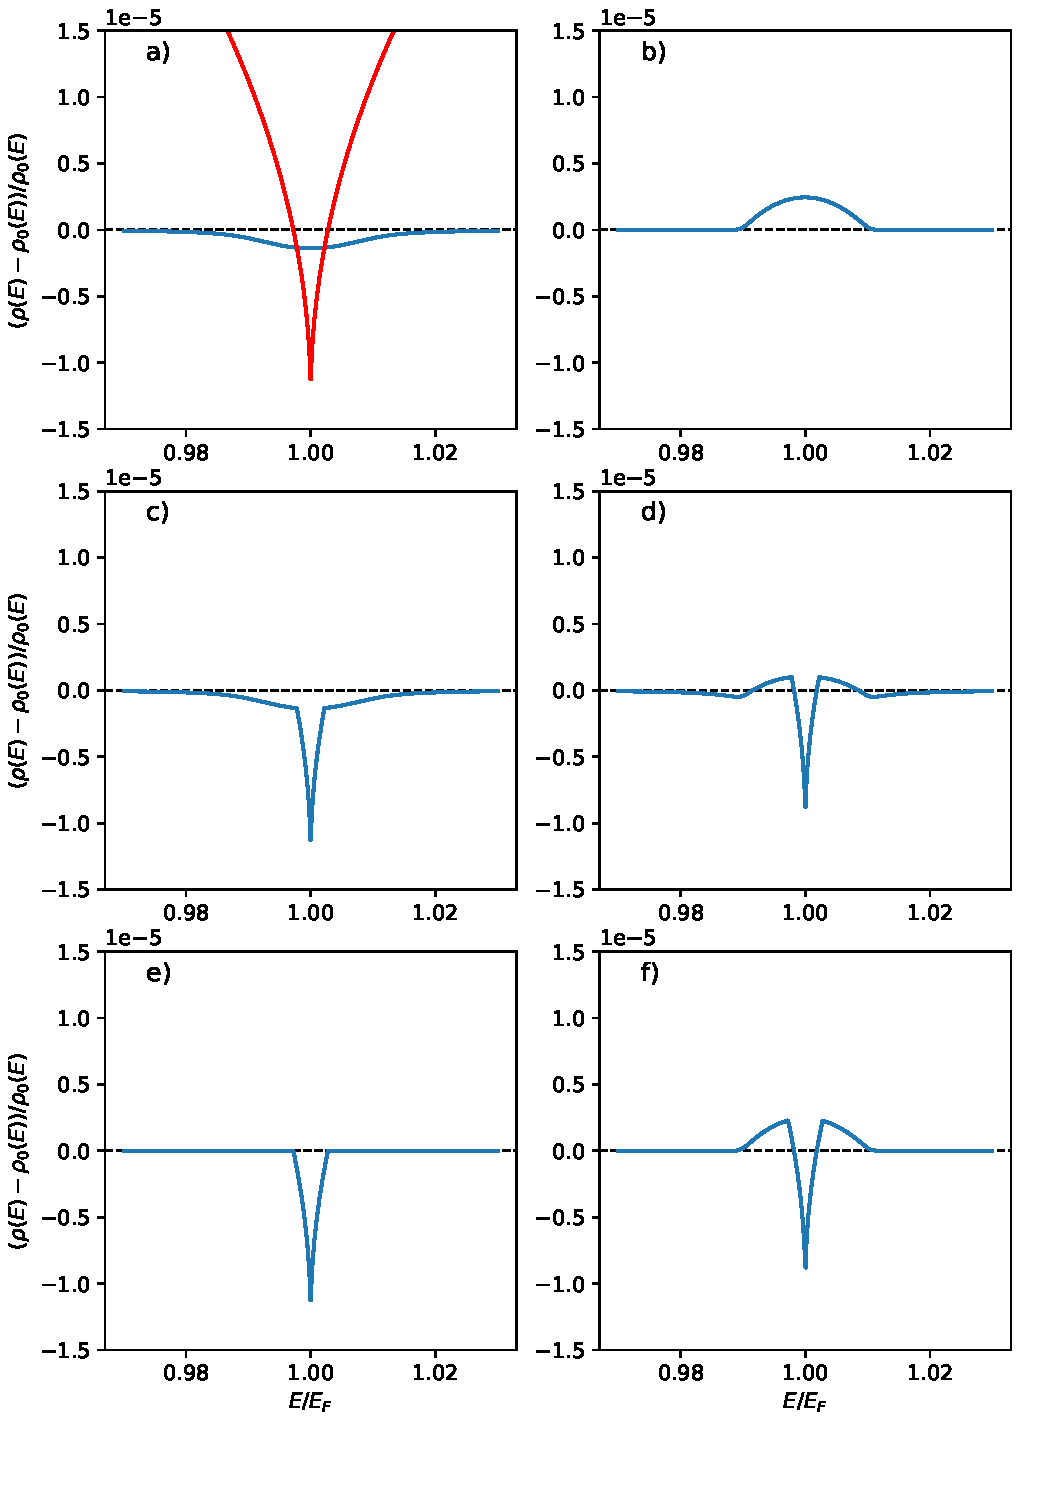
\includegraphics[scale=0.35]{grafy/plot_tau_1_c_1}
\end{column}
\begin{column}{.5\textwidth}
\small
Panel (a): Krivka ukázaná červenou farbou je pôvodná závislosť Altshulera - Aronova \eqref{eq:erg_hustota stavov relat povodny}.
krivka ukázaná modrou farbou ukazuje prvý člen numerického výpočtu \eqref{eq:erg_hustota stavov relat} . Panel (c) ukazuje obidva grafy z panelu (a) este raz, avšak "zošité" približne v energii  $|\E-\E_F| = U_{co}$. Panel (b) ukazuje druhý člen  \eqref{eq:erg_hustota stavov relat} . Panel (d) ukazuje celkovú závislosť $\frac{\rho(\E) - \rho_0(\E)}{\rho_0(\E)}$, získanú sčítaním grafov v paneloch (b) a (c).
\normalsize
\end{column}
\end{columns}
\end{frame}
\begin{frame}
\note{
Porovnanie nášho teoretickeho výsledku s experimentálnymi výsledkami. Na obrázku je vidieť kvalitatívnu podobnosť s experimentom.
}
\begin{columns}[c]
\begin{column}{.5\textwidth}
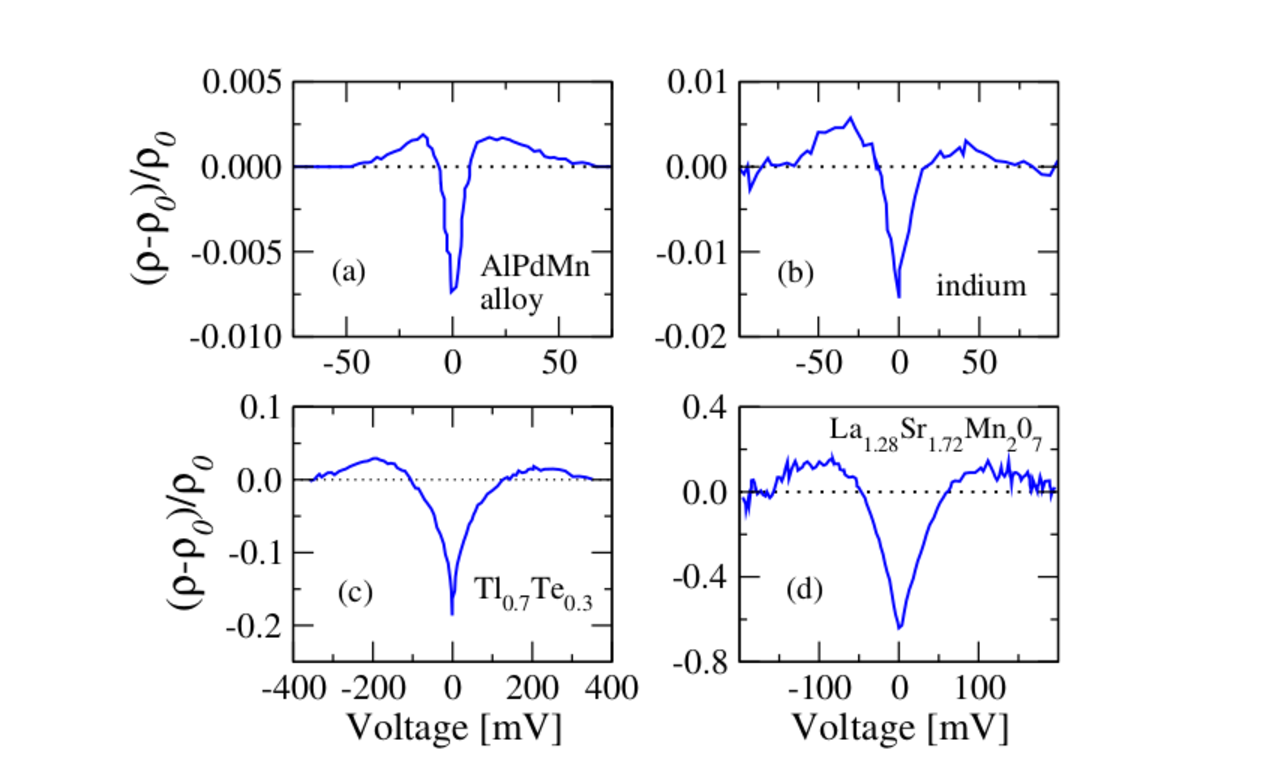
\includegraphics[scale=0.35]{grafy/B2}
\end{column}
\begin{column}{.5\textwidth}
\qquad
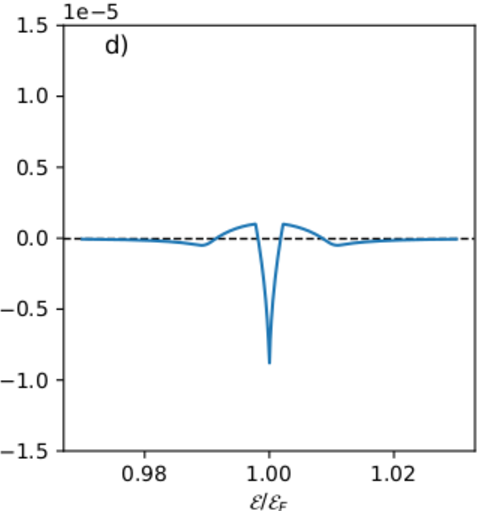
\includegraphics[scale=0.35]{grafy/final}
\end{column}
\end{columns}
Porovnanie nášho teoretickeho výsledku s experimentálnymi výsledkami. Na obrázku je vidieť kvalitatívnu podobnosť s experimentom.
\end{frame}

\begin{frame}
\frametitle{Záver}
	\begin{itemize}
	\item v tejto práci sme teoreticky študovali Altshulerov-Aronovov jav.
	\item teóriu Altshulera-Aronova, ktorá platí pre energie $|\E - \E_F| \lesssim \hbar/\tau$ sme rozšírili na energie $|\E - \E_F| \gtrsim \hbar/\tau$
	použitím self-konzistentnej Bornovej aproximácie. 
	\item Získanú hustotu stavov sme normalizovali na hustotu stavov interagujúcich elektrónov v čistom kove
	\item Získané výsledky pre relatívnu zmenu hustoty stavov sme porovnali s experimentom sme porovnali s experimentom
	\item naša teória je s experimentom v rozumnej kvalitatívnej zhode, ceníme si najmä to , že naša teória ukazuje podobné nahromadenie stavov po oboch stranách pseudogapu, ako ukazuje experiment. 
	\end{itemize}
\end{frame}
%----------------------------------------------------------------------------------------
%	CLOSING SLIDE
%----------------------------------------------------------------------------------------

\begin{frame}[plain] % The optional argument 'plain' hides the headline and footline
	\begin{center}
		{\Huge Poďakovanie}
		
		\bigskip\bigskip % Vertical whitespace
	\end{center}
Práca bola vypracovaná na Katedre experimentálnej fyziky FMFI UK a na Elektrotechnickom ústave SAV.

Moja vďaka patrí najmä môjmu školiteľovi, Doc. RNDr. Martinovi Moškovi, DrSc. za podklady a ochotu konzultovať.
Tak isto ďakujem aj mojej konzultantke RNDr. Antónii Moškovej, CSc. za odbornú pomoc. Napokon by som chcel poďakovať mojim rodičom
za podporu počas celého vysokoškolského štúdia.
\end{frame}

%----------------------------------------------------------------------------------------
%%%odpoved na otazky
\begin{frame}
\frametitle{Otázky oponenta}
Predpokladám, že veličina $\rho_0$ vo výraze $(\rho - \rho_0)/\rho_0$ na obr. 8 je rovná hustote stavov
pri pevne zvolenej energii $\E_*$, t.j. $\rho_0 = \rho(\E_*)$.

\vspace{5mm}
\textbf{Odpoveď:}\\
Nie, $\rho_0(\E)$ na obrázku 8 nie je zobraté pri konštantnej energii $\E=\E_*$. To čo sa naozaj meria je [Mazur, Phys. Rev. B, vol. 76 193102 1-4 (2007)] $$\frac{G(U)-G_0(U)}{G_0(U)}=\frac{\rho(\E)-\rho_0(\E)}{\rho_0(\E)}\text{,}$$
kde $G_0(U)$ je vodivosť bez AA efektu, ktorá väčšinou slabo závisí na $U$. Získať ju experimentálne nie je jednoduché [Mazur, PR B, 2007]
\vspace{5mm}
 
Tí experimentátori, ktorí chcú vidieť len AA pseudogap v blízkosti $E_F$, niekedy naozaj používajú normu $G(U)/G_0(U_*)$. 
\end{frame}
\begin{frame}
\frametitle{Otázky oponenta}

 Na druhej strane, výsledky prezentované na obr. 10-12 sú vztiahnuté vzhľadom ku (v princípe) energeticky závislej funkcii
$\rho_0(\E)$. Možno na energetických škálach používaných v obr. 10-12 túto závislosť zanedbať. Inými slovami, ako vyzerajú grafy $[\rho_0(\E)-\rho_0(\E_*)]/\rho_0(\E_*)$ pre $\E_*$ rovné povedzme
maximálnym energiám v obr. 10-12?
\end{frame}
\begin{frame}
\frametitle{Otázky oponenta}
\begin{figure}%
    \centering
    \subfloat{{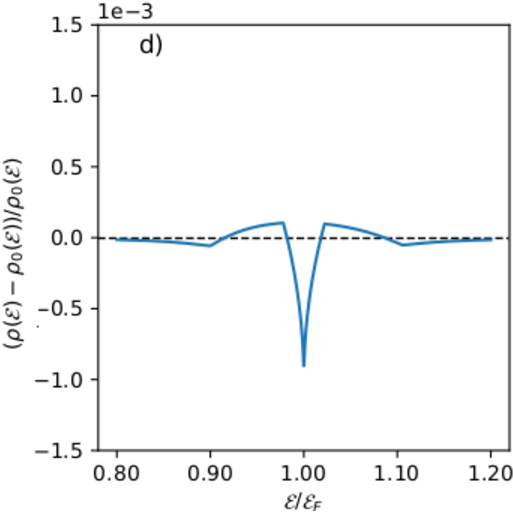
\includegraphics[scale=0.3]{grafy/obrazok_obhajoba_1} }}%
    \\
    \subfloat{{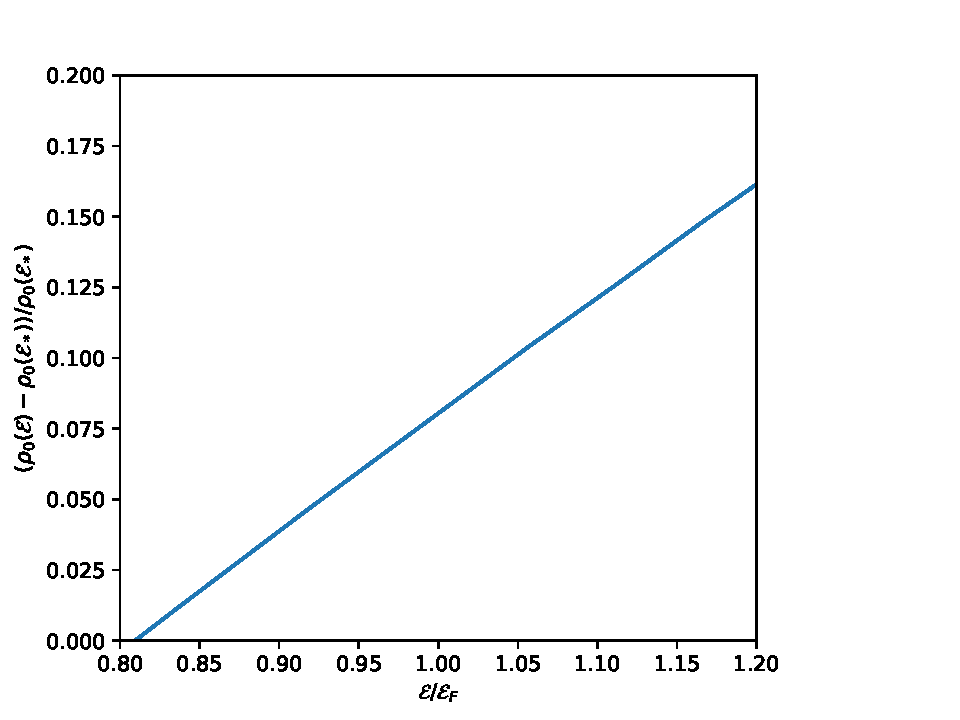
\includegraphics[scale=0.3]{grafy/obrazok_obhajoba_2} }}%
      \subfloat{{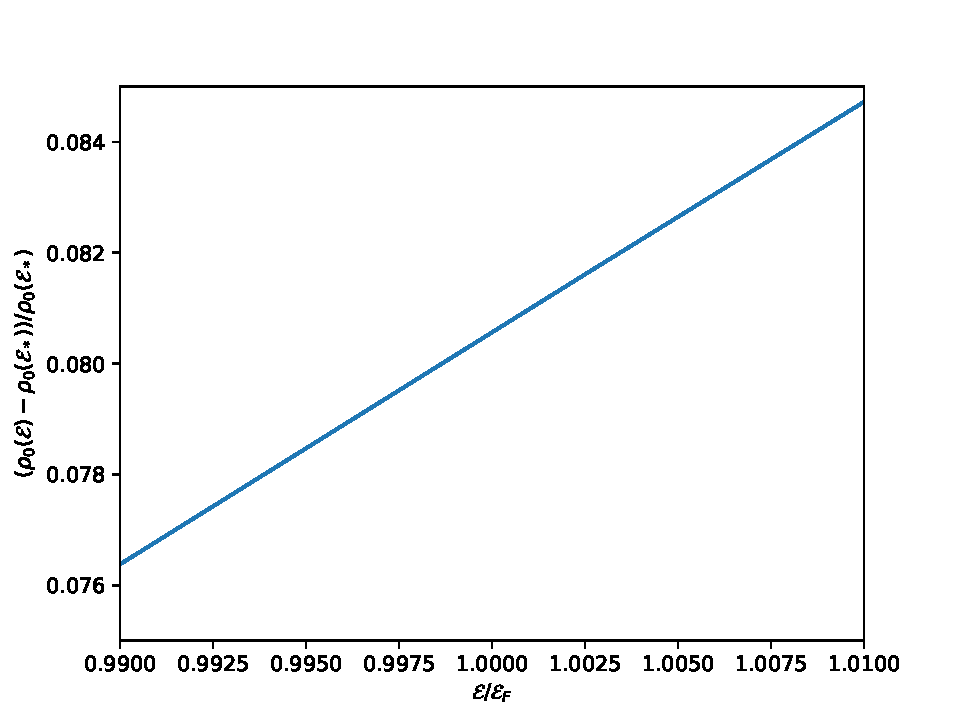
\includegraphics[scale=0.3]{grafy/obrazok_obhajoba_3} }}%
    \vspace{-10mm}
    \label{fig:example}%
\end{figure}
\end{frame}
\begin{frame}
\frametitle{Otázky oponenta}

Ako by vyzerali výsledky prezentované na obr. 10-12, keby sme priamo vykresľovali
experimentálne relevantnú veličinu $[\rho(\E)-\rho_0(\E_*)]/\rho_0(\E_*)$?
\vspace{5mm}
\textbf{Odpoveď:}\\
V práci som plotoval
$$\frac{\rho(\E)-\rho_0(\E)}{\rho_0(\E)}=f(\E)$$
Oponent chce vidieť:
$$\frac{\rho(\E)-\rho_0(\E_*)}{\rho_0(\E_*)} = f(\E)\frac{\rho_0(\E)}{\rho_0(\E_*)}+\frac{\rho_0(\E)}{\rho_0(\E_*)} - 1$$
\end{frame}
\begin{frame}
\frametitle{Otázky oponenta}
\begin{figure}%
    \centering
    \subfloat{{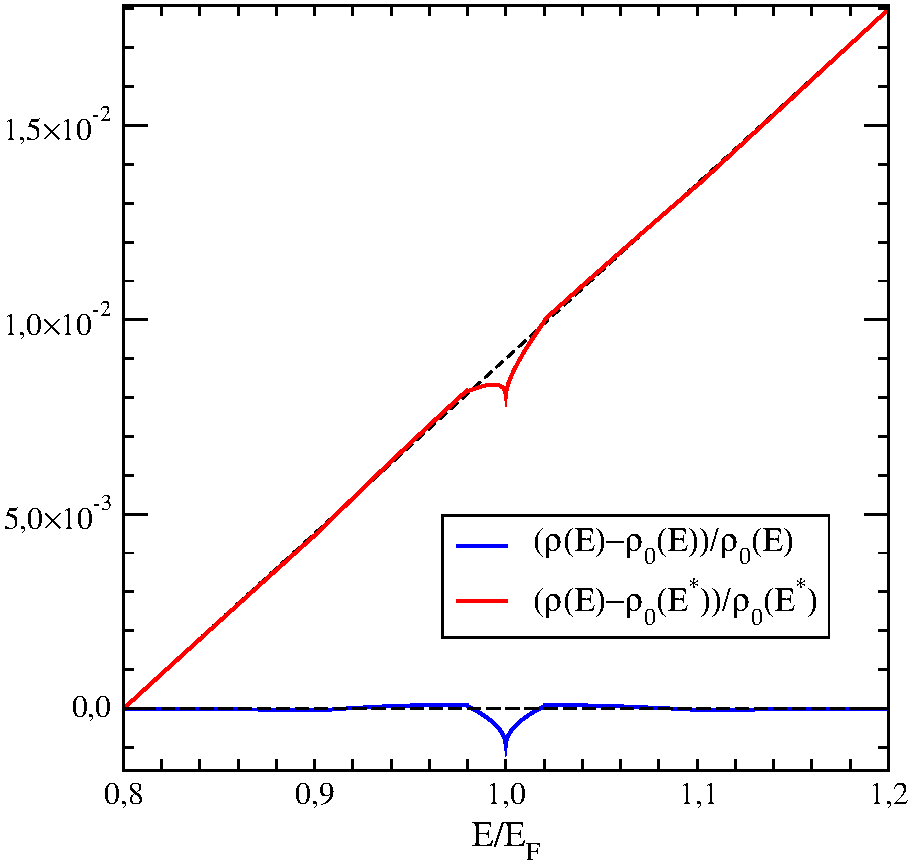
\includegraphics[scale=0.4]{grafy/figTTobhajoba} }}%
    \subfloat{{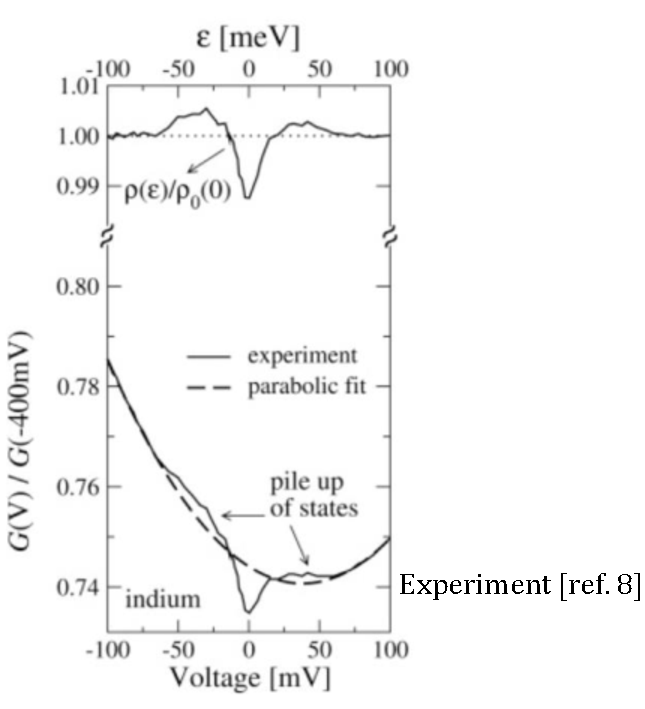
\includegraphics[scale=0.5]{grafy/obhajobaExperimental} }}%
    \vspace{-10mm}
    \label{fig:example}%
\end{figure}
\end{frame}
\begin{frame}
\frametitle{Otázky oponenta}
Je veličina $\rho_0(\E)$, na ktorú sú normalizované výsledky v kapitole 4, totožná s normalizačnou hustotou stavov danou vzťahom (64) v kapitole 2? Ovplyvní táto skutočnosť
konštrukciu sumárnych grafov 10c a 10d (a podobne pre obr. 11 a 12)?

\vspace{5mm}
\textbf{Odpoveď:}\\
Nie, veličina $\rho_0(\E)$ v kapitole 4 obsahuje e-e interakciu, zatiaľ čo veličina $\rho_0(\E)$ vo vzťahu (64) je hustota stavov neinteragujúcich elektrónov. Táto skutočnosť neovplyvní konštrukciu sumárnych grafov na obrázkoch 
10, 11 a 12, pretože člen $\frac{dE^{AA}_{self}(\E)}{d\E}$ v rovnici (135) od  normalizácie nezávisí. 

\vspace{5mm}
Náš spôsob normalizácie by sa dal do AA odvodenia v kapitole 2 ľahko dorobiť tak, že by sa do hranatej zátvorky rovnice (79) pridal člen $\frac{dE^{free}_{self}(\E)}{d\E}$. Tento člen by AA závislosť len rigidne posunul smerom hore, dá sa to vidieť aj na našich obrázkoch.
\end{frame}
\begin{frame}
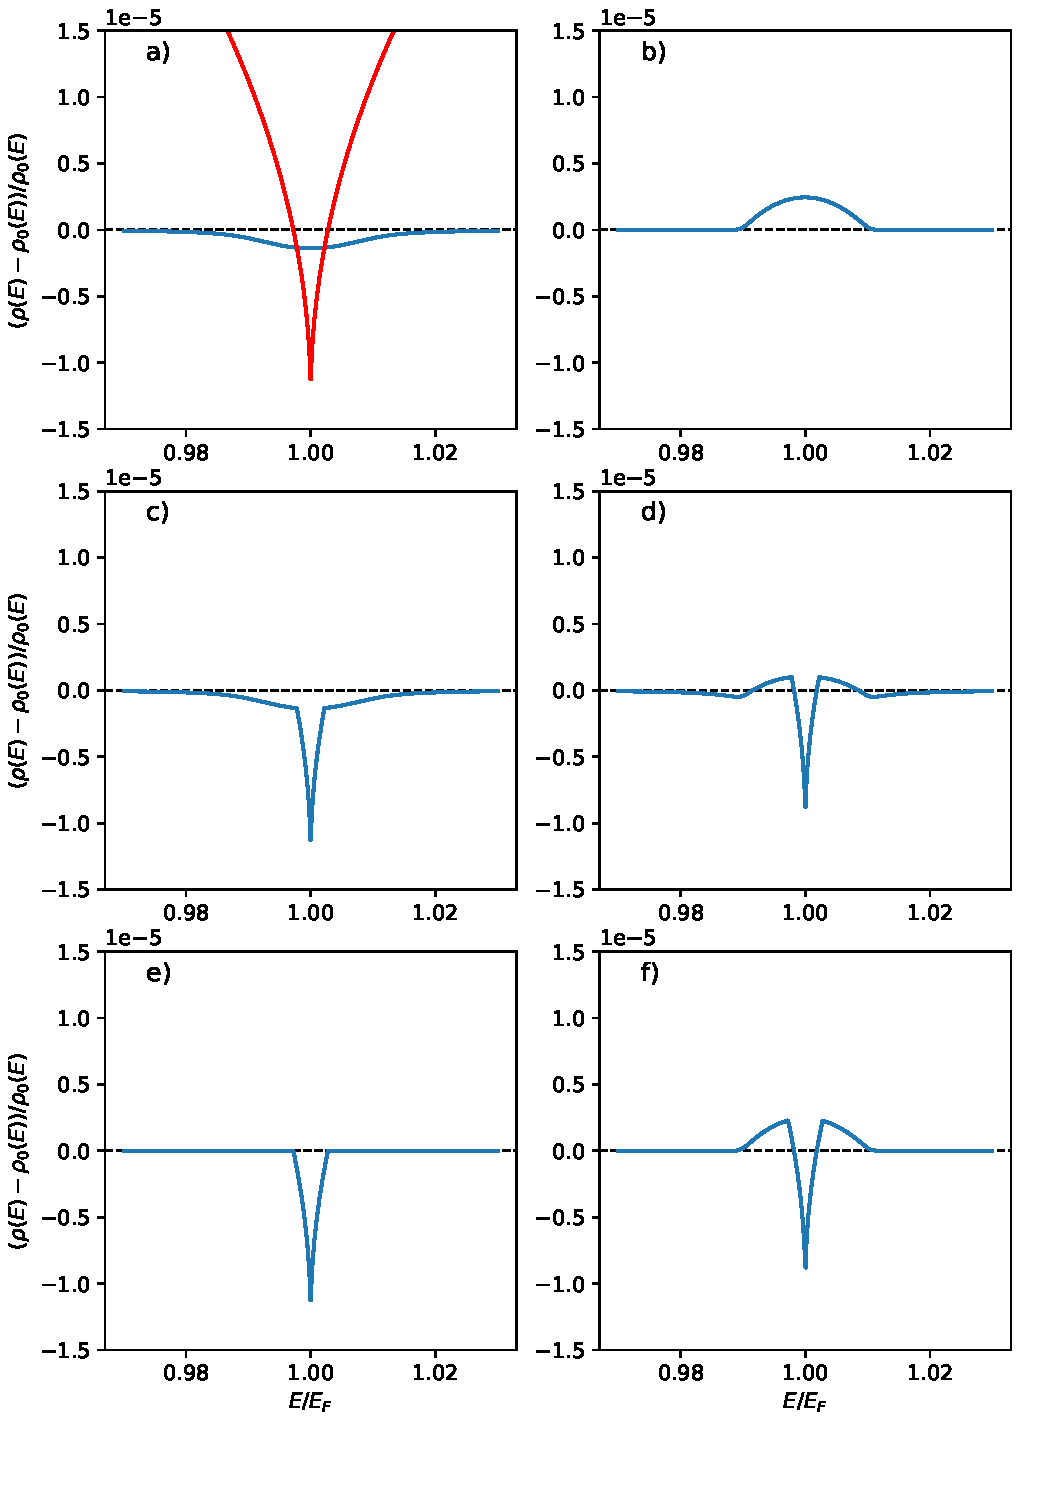
\includegraphics[scale=0.5]{grafy/plot_tau_1_c_1}
\end{frame}
\begin{frame}
\frametitle{Otázky oponenta}
 V staršej práci školiteľa a konzultantky [21] sa ukazuje, že celkový počet stavov v
experimentálnych systémoch so singularitou Aľtšulera-Aronova sa zachováva už na
škálach porovnateľných s $\hbar/\tau$. Dá sa tento výsledok zdôvodniť v rámci navrhovaného
prístupu?

\vspace{5mm}
\textbf{Odpoveď:}\\
Upresníme, že experimentálne merania, napríklad dáta v paneli \emph{d} obrázku 8 neukazujú exaktné zachovanie stavov, ale len 80 \%-né. Experimentátori ale veria, že za tých 80\% môže byť zodpovedná nepresnosť merania  [Mazur, PR B, 2007]. Práca [21] vychádzala z predpokladu, že stavy sa budú zachovávať presne. V našej práci nerobíme o zachovaní stavov žiadny predpoklad a nevieme povedať, či nám nakoniec výjde zachovanie stavov. V súčasnom štádiu výpočtov to tak nevyzerá, zatiaľ nás teší len kvalitatívna podobnosť vypočítaných a nameraných grafov.
\end{frame}
\begin{frame}
\frametitle{Otázky oponenta}
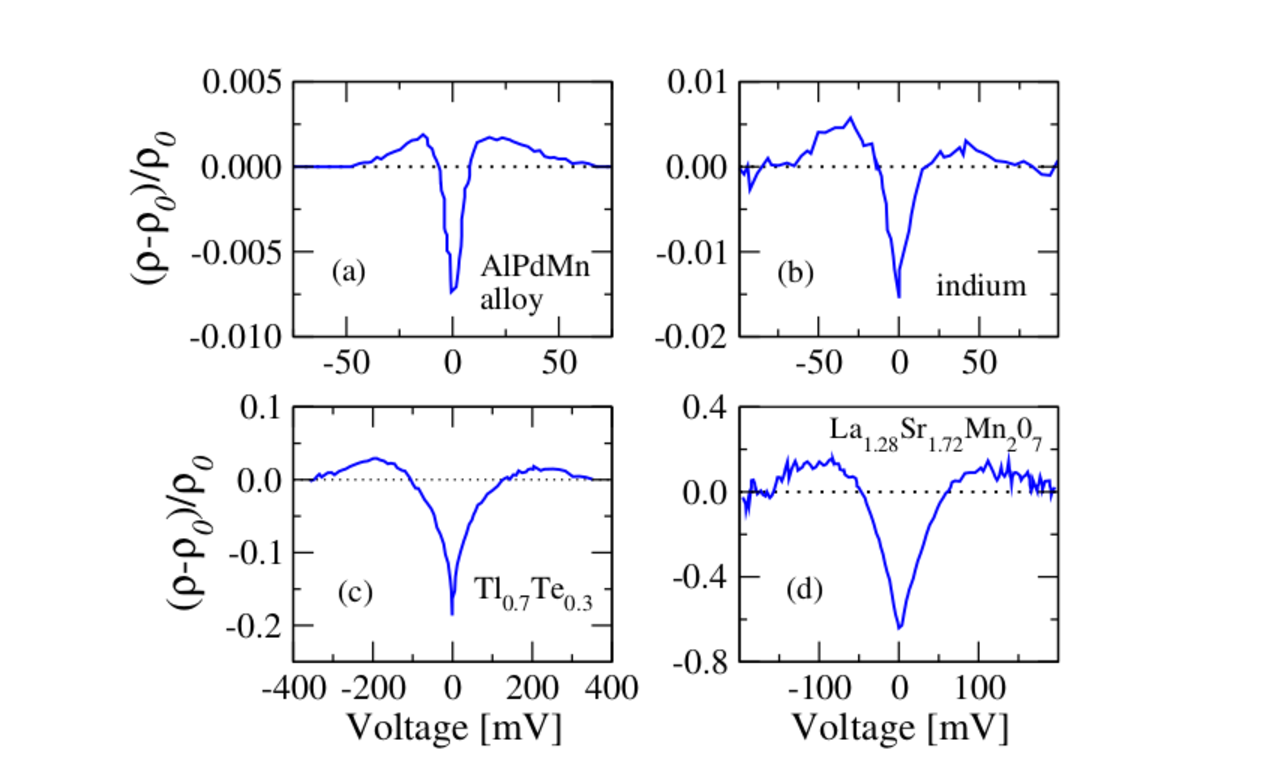
\includegraphics[scale=0.5]{grafy/B2}
\end{frame}
\begin{frame}
\centering
\Huge{Ďakujem za pozornosť}
\end{frame}
%%%%%%%%%%%%%%%%%%%%%%%%%%%%%%%%%%%
%NAHRADNE SLIDY

%%%%%%%%%%%%%%%%%%%%%%%%%%%%

\begin{frame}
\frametitle{Otázky oponenta}
\begin{figure}%
    \centering
    \subfloat{{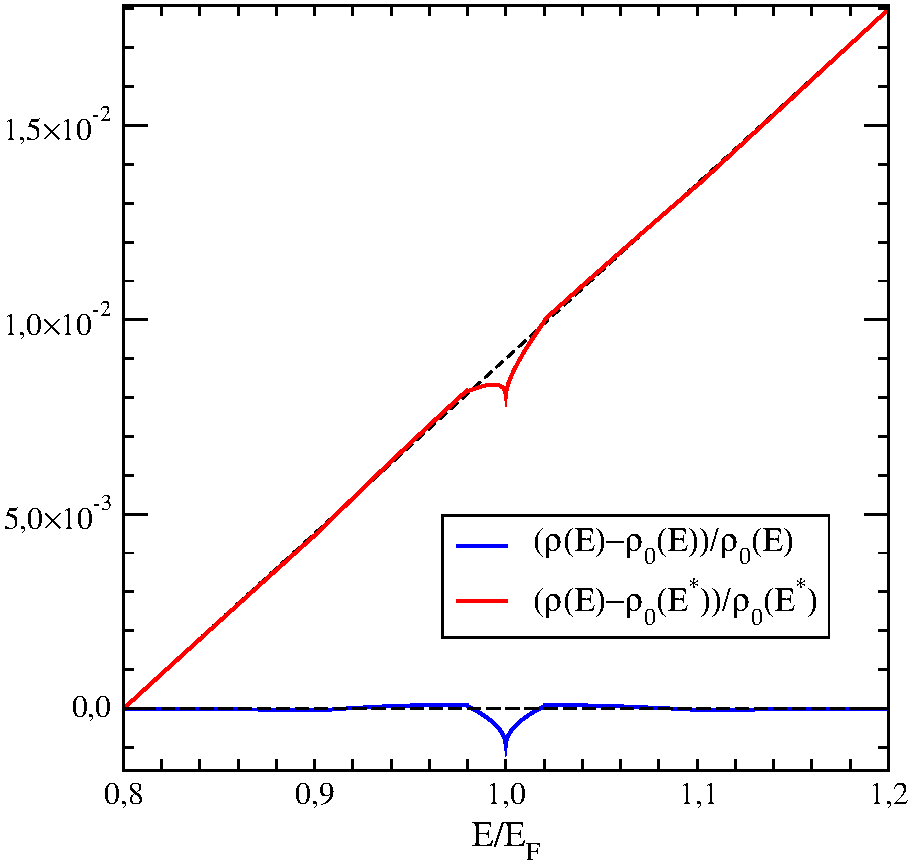
\includegraphics[scale=0.4]{grafy/figTTobhajoba} }}%
    \subfloat{{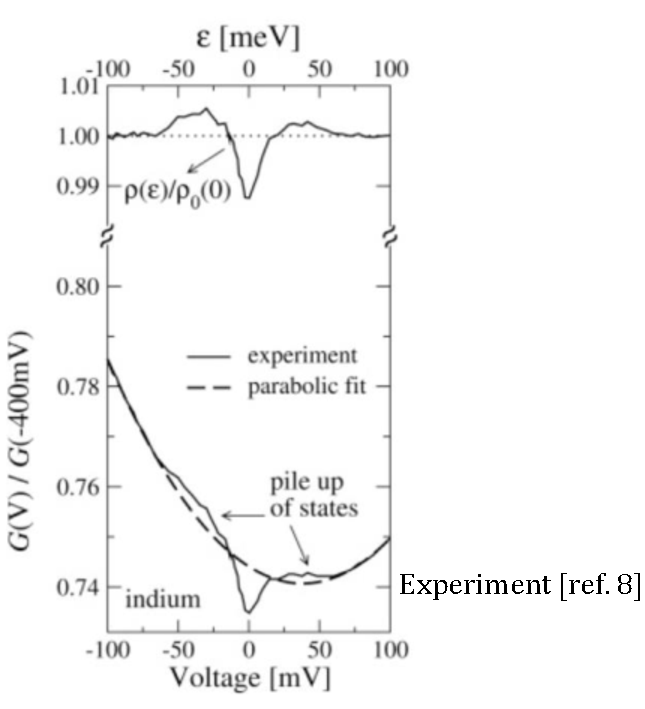
\includegraphics[scale=0.5]{grafy/obhajobaExperimental} }}%
    \vspace{-10mm}
    \label{fig:example}%
\end{figure}
\end{frame}


\begin{frame}
Výsledná energia interagujúcich elektrónov v čistom kove v Hartree-Fockovom priblížení:
\begin{equation}
\label{eq:fock_erg}
E(k)=\frac{\hbar^2 k^2}{2m}- \frac{e^2 k_f}{4\pi^2\epsilon_0} F(\frac{k}{k_f})\ \ \text{kde}\ \ F(x)=\frac{1}{2}+\frac{1-x^2}{4x}\ln{\frac{|1+x|}{|1-x|}} \text{.}
\end{equation}

\begin{figure}%
    \centering
    \subfloat{{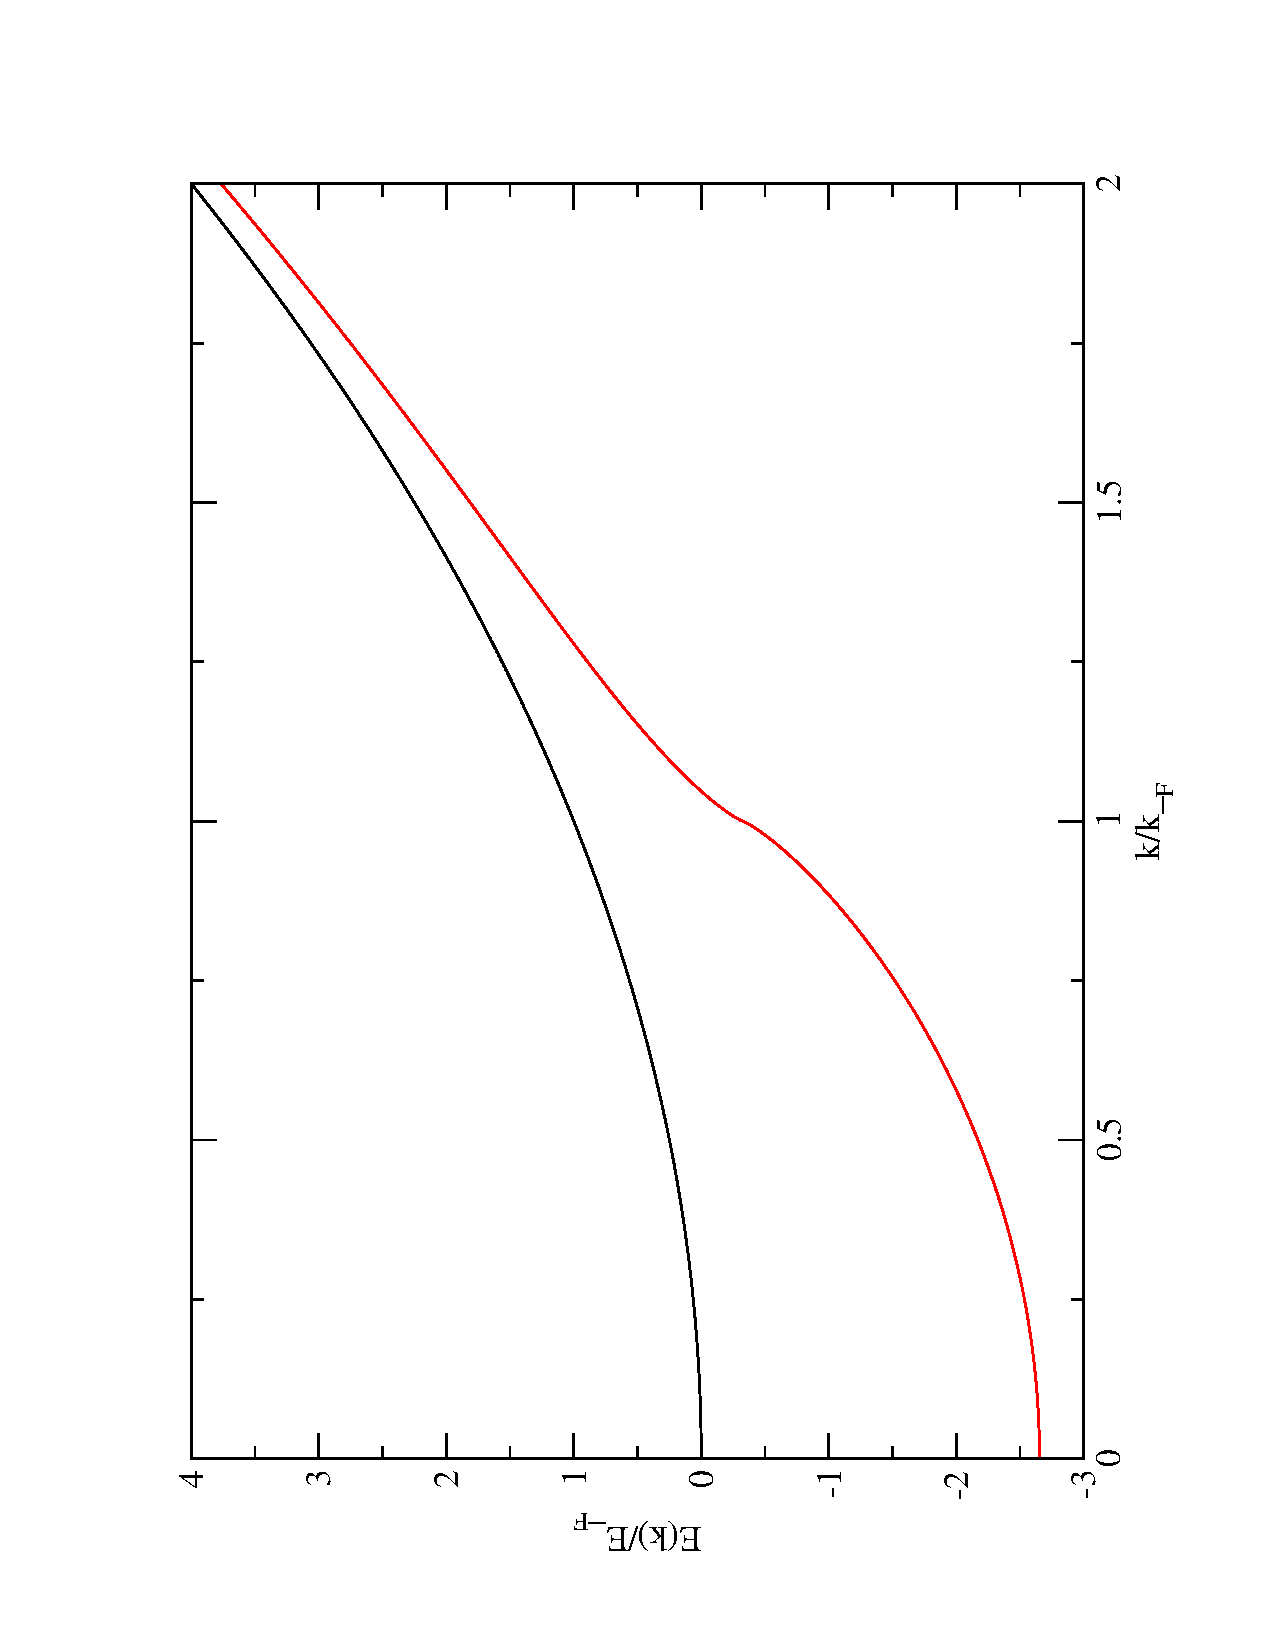
\includegraphics[angle=-90,origin=c,scale=0.2,trim={1cm 0 1cm 0},clip]{grafy/hartree_erg} }}%
    \subfloat{{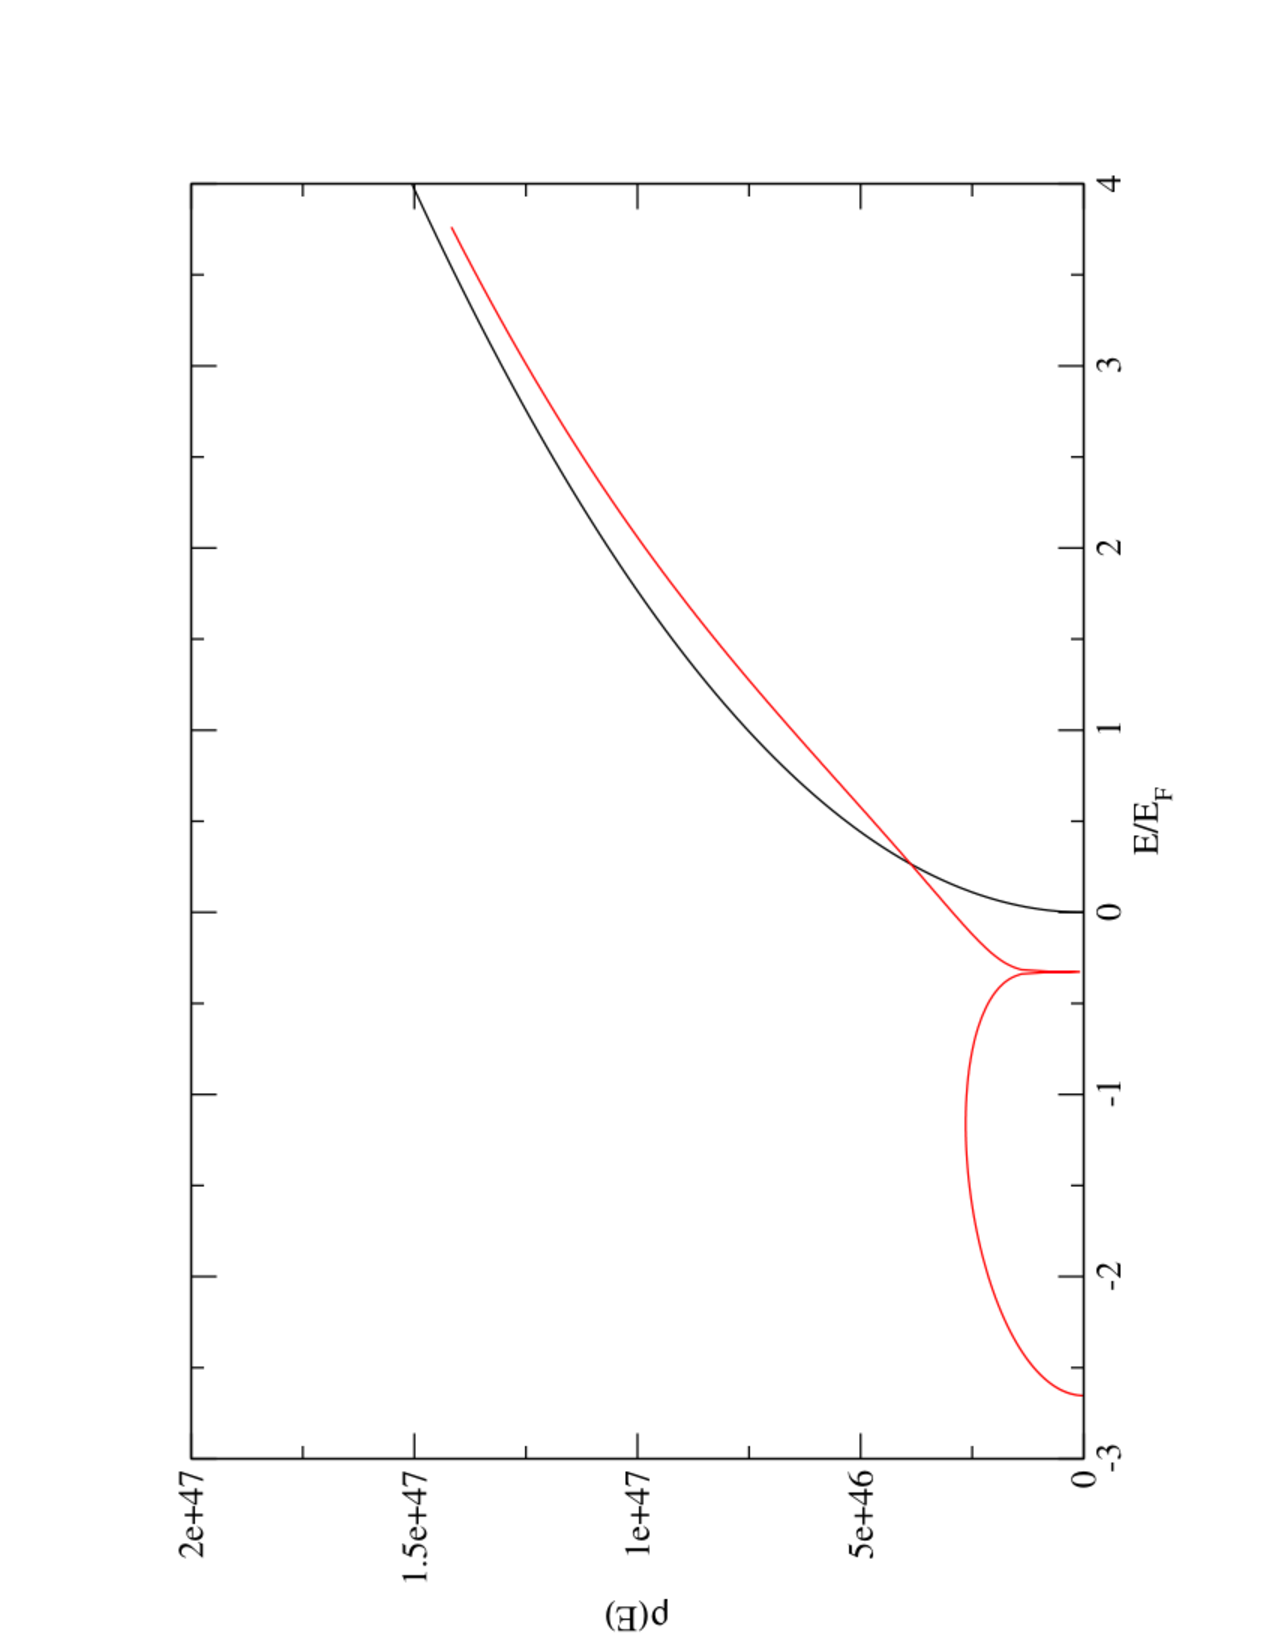
\includegraphics[angle=-90,origin=c,scale=0.2,trim={1cm 0 1cm 0},clip]{grafy/hartree_dos_NEW} }}%
    \vspace{-10mm}
    \label{fig:example}%
\end{figure}
\small
    Vľavo je energia podľa rovnice \eqref{eq:fock_erg}. V pravo hustota stavov prislúchajúca \eqref{eq:fock_erg}. Na pravom obrázku vidíme singularitu v novej hodnoty Fermiho energie, čo znamená že HF aproximácia je v pre holý Coulombovský potenciál v rozpore s realitou. Hustota stavov na novej hodnote Fermiho energie je totiž nulová, v takomto prípade by bol každý kov izolant.%
    \normalsize
\end{frame}

\begin{frame}
\begin{itemize}
\item  Zavedieme bezrozmerné premenné a konštanty:
\small
\begin{equation}
w=\frac{\epsilon_m}{\epsilon_\tau} \ \ \text{,} \ \
u=\frac{\epsilon_{m'}}{\epsilon_\tau} \ \ \text{,} \ \
x=\frac{\epsilon_k}{\epsilon_\tau} \ \ \text{,} \ \
y=\frac{\epsilon_q}{\epsilon_\tau} \ \ \text{,} \ \
\bar{y}=\frac{q}{k_s}  \ \   \text{,} \ \
\bar{y}_{max}=\frac{q_{max}}{k_s}  \ \ \text{,} \ \
u_{EF}=\frac{\E_F}{\epsilon_\tau}  \ \ \text{.}
\end{equation}
\normalsize
\item Po vykonaní analytických integrálov dostaneme
\begin{align}
\label{eq:05energy6}
E_{self}^{AA}(\epsilon_m)= -\frac{e^2}{4\pi^4\epsilon_0 k_s^{-1}} \int_0^{\bar y_{max}} d\bar{y}\ \frac{\bar{y}^2}{1+\bar{y}^2}\int_0^{\infty} dx \frac{1}{(w-x)^2+1}F(x,y) \text{,}
\end{align}
kde
\tiny
\begin{align*}
F(x,y)=\frac{1}{\sqrt{4xy}}& \{(x+y+2\sqrt{xy}-u_{EF})\arctan(x+y+2\sqrt{xy}-u_{EF}) \\
&-(x+y-2\sqrt{xy}-u_{EF})\arctan(x+y-2\sqrt{xy}-u_{EF}) \\
&-(x+y+2\sqrt{xy})\arctan(x+y+2\sqrt{xy}) \\
&+(x+y-2\sqrt{xy})\arctan(x+y-2\sqrt{xy}) \\
&-\frac{1}{2}ln(\frac{(x+y+2\sqrt{xy}-u_{EF})^2+1}{(x+y-2\sqrt{xy}-u_{EF})^2+1}\ \frac{(x+y+2\sqrt{xy})^2+1}{(x+y-2\sqrt{xy})^2+1})\}\text{.}
\end{align*}
\normalsize
\item Integrály \eqref{eq:05energy6} počítame numericky obdĺžnikovou metódou
\end{itemize}
\end{frame}
\end{document} 